\documentclass[11pt]{labbook}
\usepackage[utf8]{inputenc}
\usepackage{graphicx}
\usepackage[margin=1.0in]{geometry}
\usepackage{setspace}
\usepackage{listings}
\usepackage{color}
\usepackage{array}
\usepackage{amsmath}
\usepackage{float}
\usepackage{verbatim}
\usepackage[final]{pdfpages}
\usepackage{caption}
\usepackage{subcaption}
\usepackage{algpseudocode}
%%%%%%%%%%%%%%% Section for new commands %%%%%%%%%%%%%%%%%%%
\newcommand{\Loss}[2]{L\left(#1,#2\right)}

%%%%%%%%%%%%%%% End %%%%%%%%%%%%%%%%%%%%%%%%%%%%%%%%%%%%%%%%

\title{Lab Notebook}
\author{Alex Cope}
\date{August 2016}



\begin{document}
\maketitle
\let\cleardoublepage\clearpage
\tableofcontents
\labday{Grant Writing notes}
\experiment{NSF Proposals by David Smelser}
\subexperiment{What does OSP do?}
Review proposals for compliance w/ federal, state, etc policies/regulations

Reviews all documents within proposal

provides feedback

Average NSF proposal is 60 pages

https://osp.utk.edu/
\subexperiment{Cayuse SP}
Tells institution as whole what you're working on (especially concerned with intellectual property)
Once sections complete and submitted, notifies Department and college the the proposal needs to be approved
Should arrive in OSP bt  business days before submission date. 
Wilhelm says it takes him over an hour

\subexperiment{Single copy documents}
List of all people you have worked with in your career, including on projects, papers, textbooks, etc.
Always evolving document.
Lifetime conflict with advisors.
Post-doctoral sponsors no longer officially considered in conflict.
Sometimes, you have to look into pubmed to find where people work.
Wilhelm says this is changing so a conflict is only between senior author and first author.
Can petition to have certain people not review proposal based on things like completely opposite views on the science involved.

\subexperiment{Project summary}
One page, no more than that
Overview, statement of intellectual merit, statement on broader impact
Write in 3rd person
Should not be an abstract

\subexperiment{Biosketches}
Should change to best reflect products most closely related to project proposal

Ex) If want funding for REU, maybe include papers that had undergraduate authors

Have any further questions, contact David Smelser at dsmelser@utk.edu
\labday{Mathematics and Statistics Notes}
 

\experiment{Chapter 7: Model Assessment and Selection}
Taken from \textit{The Elements of Statistical Learning}, 2nd ed, Hastie et al.
\subexperiment{7.2 Bias, Variance, and Model Complexity}
 
Let L(Y,$\hat{f}$(X)) be a loss function (can be squared error, absolute, etc), with X being a vector input, Y being a target vector, and $\hat{f}$(X) being estimated from some training set. Let $\mathcal{T}$ represent a training set. Then the test error is

\begin{align*}
Err_\mathcal{T} &= E\left[L\left(Y,\hat{f}(X)\right)|\mathcal{T}\right]
\end{align*}

which is the prediction error over an independent sample. Note that X and Y are drawn from their joint distribution. The expected test error is 

\begin{align*}
Err &= E\left[L\left(Y,\hat{f}(X)\right)\right] = E\left[Err_\mathcal{T}\right]
\end{align*}

Err is better for statistical analysis and most methods estimate this quantity. 
\newline

Training error:

\begin{align*}
\overline{err} &= \frac{1}{N}\sum_{i=1}^{N}\Loss{y_i}{\hat{f}(x_i)}
\end{align*}


As model complexity increases, training data is used more and adapts to more complicated information extracted from the model; however, this drives down the bias but increases the variance. Want to minimize expected test error. 

Training error is not a good estimate of test error. In fact, a model with a training error of 0 is an overfit, meaning it will perform poorly when working with other data sets. 

What if we are working with categorical data. The situation is very much the same. Let $\Loss{G}{\hat{G}(X)}$ (G = $\hat{G}$(X) = $argmax_k$ $\hat{p}_k$(X)) be a loss function, where G is a categorical response taking one of K values. Let $p_k(x)$ be the probability that G = k given the input X. A loss function in this case might be 0-1 loss or something more complex (see pg. 221).

Training error for this type of data is 

\begin{align*}
\overline{err} = -\frac{2}{N}\sum_{i=1}^{N}log\hat{p}_{g_i}(x_i)
\end{align*}

The log-likelihood can serve as a loss-function for Poisson, gamma, exponential, and log-normal. From my understanding, this is essentially what ROC and similar models do when sampling gene expression values. Let $Pr_{\theta\left(X\right)}$(Y) be the density of Y, indexed by $\theta$(X), then

\begin{align*}
\Loss{Y}{\theta(X)} &= -2 \cdot logPr_{\theta\left(X\right)}(Y)
\end{align*}

\subexperiment{7.3 The Bias-Variance Decomposition} 
Let Y = f(X) + $\epsilon$, where the average value of $\epsilon$ is 0 and the variance is equal to $\sigma_\epsilon^2$. Then with a regression $\hat{f}$(X) at point $x_0$ with squared error loss, the expected prediction error is 

\begin{align*}
Err(x_0) &= Irreducible Error + Bias^2 + Variance
\end{align*}

where the first term is the variance of the target around true mean f($x_0$), the second is the amount by which the estimate differs from the true mean, and the third is the expected squared deviation of $\hat{f}(x_0)$ around its mean. Generally, the more complex $\hat{f}$, the lower the squared bias but the higher the variance. 

The biggest thing to take from this section is that as model complexity goes up, squared bias generally decreases, but variance increases. 


\subexperiment{7.4 Optimism of the Training Error Rate}
Typically, the training error is less than the true error because same data used to fit and assess the model. 

Define the \textit{in-sample error} to be
\begin{align*}
Err_{in} &= \frac{1}{N}\sum_{i=1}^{N}E_{Y^0}\left[\Loss{Y_i^0}{\hat{f}(x_i)}|\mathcal{T}\right]
\end{align*}

$Y^0$ indicates N new responses for N training points. Let the \textit{optimism} and its corresponding average over training sets \textbf{y}, $\omega$, be
\begin{align*}
op \equiv Err_{in} -\overline{err} \\
\omega \equiv E_{\textbf{y}}(op)
\end{align*}
which is usually a positive term since the training error is usually driven down by fitting/assessment approach. Usually can only estimate $\omega$. For many common loss functions (including squared error),

\begin{align*}
\omega &= \frac{2}{N}\sum_{i=1}^{N}Cov\left(\hat{y}_i,y_i\right)
\end{align*}
In summary, the expected value of the in-sample error is the sum of expected value of the training error over training sets \textbf{y} and $\omega$,
\begin{align*}
 E_{\textbf{y}}(Err_{in}) &= E_{\textbf{y}}(\overline{err}) + \frac{2}{N}\sum_{i=1}^{N}Cov\left(\hat{y}_i,y_i\right)
\end{align*}   

If $\hat{y}_i$ is obtained via linear fit with d inputs, then,
\begin{align*}
\sum_{i=1}^{N}Cov\left(\hat{y}_i,y_i\right) &= d\sigma_{\epsilon}^{2} \\
\rightarrow  E_{\textbf{y}}(Err_{in}) &= E_{\textbf{y}}(\overline{err}) + 2 \cdot \frac{d}{N}\sigma_{\epsilon}^{2}
\end{align*}
Optimism increases linearly with number of inputs, but decreases as training set increases in size. 

\subexperiment{7.5 Estimates of In-Sample Prediction Error}
Let d parameters be fit under squared error loss, then you get the $C_p$ statistic,
\begin{align*}
C_p &= \overline{err} + 2 \cdot \frac{d}{N}\hat{\sigma}_{\epsilon}^{2}
\end{align*}

Note: $\hat{\sigma}_{\epsilon}^{2}$ is estimate of the noise variance.
\newline
\newline
\textbf{Akaike information criterion (AIC)}:\newline

Used to estimate $Err_{in}$ when using log-likelihood loss function. 

\begin{align*}
-2 \cdot E\left[logPr_{\hat{\theta}}(Y)\right] &\approx -\frac{2}{N} \cdot E\left[loglik\right] + 2 \cdot \frac{d}{N} \\
\hat{\theta} &= MLE(\theta) \\
loglik &= \sum_{i=1}^{N}logPr_{\hat{\theta}}(Y)
\end{align*}

where $Pr_{\theta}$(Y) is a family of densities for Y (one of which is the true density).

When selecting a model via AIC, choose one that minimizes AIC. It is important to note that when using nonlinear models, d must be replaced with some measurement of model complexity. 

In general, let $\mathcal{F}$ be a set of models $f_{\alpha}$(x), where $\alpha$ is a tuning parameter. Then,
\begin{align*}
AIC(\alpha) &= \overline{err}(\alpha) + 2 \cdot \frac{d(\alpha)}{N}\hat{\sigma}_{\epsilon}^2
\end{align*}
Basically, AIC estimates the test error curve, so you want to find the $\hat{\alpha}$ that minimizes it. 

Book notes that if basis functions are chosen adaptively, this whole thing collapses. 
\newline

Example) You have p total inputs, but best fitting linear model takes $d<p$ inputs, optimism will exceed (2d/N)$\sigma_{\epsilon}^{2}$.

\subexperiment{7.7 The Bayesian Approach and BIC}
Like AIC, applicable where fitting occurs via maximizing log-likelihood. Generic form of BIC:

\begin{align*}
BIC &= -2 \cdot loglik + \left(log N\right) \cdot d
\end{align*}

Under a Gaussian model ($\sigma_{\epsilon}^2$ is known), $-2 \cdot loglik$ equals up to a constant $\sum_i^N(y_i -\hat{f}(x_i))/\sigma_{\epsilon}^2$. For a squared error loss, this is $N \cdot \overline{err}/\sigma_{\epsilon}^2$
\begin{align*}
\rightarrow BIC &= \frac{N}{\sigma_{\epsilon}^2}\left[\overline{err} + \left(log N\right) \cdot \frac{d}{N}\sigma_{\epsilon}^2\right] \\
\rightarrow BIC &\propto AIC
\end{align*}

BIC tends to penalize complex models, but as $N \rightarrow \infty$, the probability BIC picks correct model goes to 1.



\experiment{Chapter 6: Model Checking}
\subexperiment{6.1 The place of model checking in applied Bayesian statistics}

\textit{Sensitivity Analysis} - how much do posterior inferences change in our model versus other models

\subexperiment{6.2 Do the inferences from the model make sense?}

\underline{Checking model via external validation} \newline
$\bullet$	Use model to make predictions, collect actual data, do they match up? \newline
$\bullet$ Usually need to check model \textbf{before} getting new data

\subexperiment{6.3 Posterior predictive checking}

To measure discrepancy between models and data, define test quantity T(y,$\theta$). Think test statistic in frequentist hypothesis testing, which depends only on data. To measure lack of fit of data with respect to posterior predictive distribution can be measured as p-value of test quantity. In a Bayesian framework, the p-value is 

\begin{align*}
p_B &= Pr(T(y^{rep},\theta) \geq T(y,\theta)|y)\\
&= \iint{I_{T(y^{rep},\theta) \geq T(y,\theta)}p(y^{rep}|\theta)p(\theta|y)dy^{rep}d\theta}
\end{align*}

which translates to the probability a set of replicated data could be more extreme than the observed (\textbf{how is this different from the frequentist's definition?}). A p-value can be calculated via simulations: drawing from joint posterior distribution, the p-value is simply the ration of

\begin{align*}
T(y^{rep s},\theta) \geq T(y,\theta^s)
\end{align*}

where the $y^{rep s}$ are drawn from the simulated values of $\theta^s$.

\experiment{Chapter 7: Evaluating, comparing, and expanding models}

\subexperiment{7.1 Measures of predictive accuracy}
Measures of predictive accuracy should be guided by the application:
$\bullet$ point prediction - single value reported as prediction of future observation (mean squared error)
\newline
$\bullet$ probabilistic prediction - report inferences about $\tilde{y}$ that takes into account full uncertainty over $\tilde{y}$
\newline

Log-likelihood, $\log{p(y|\theta)}$, is a probabilistic prediction. Proportional to the mean squared error if model is normal with constant variance. With large sample sizes, minimizing Kullback-Leibler information is the same as maximizing expected log-likelihood. Use log-likelihood because of its generality and because we are interested in summarizing the model fit to data (prior density is not relevant in computing predictive accuracy). 
\newline
\newline
\underline{Ideal measure of model fit: predictive performance for new data (external validation).} 
\newline

Let:\newline
$\bullet$ f be the true model \newline
$\bullet$ y be the observed data \newline
$\bullet$ $\tilde{y}$ be the future/alternative data

Out-of-sample predictive fit for new data point $\tilde{y}_i$ is
\begin{align*}
\log{p_{post}(\tilde{y}_i)} &= \log{E_{post}(p(\tilde{y}_i|\theta))}\\
&= \log{\int p(\tilde{y}_i|\theta)p_{post}(\theta)d\theta}
\end{align*}
where $p_{post}(\tilde{y}_i$ is the predictive density and $p_{post}(\theta)$ is the posterior. 

Expected out-of-sample log-likelihood, since future data unknown:
\begin{align*}
E_f(\log{p_{post}(\tilde{y}_i)}) &= \int(\log{p_{post}(\tilde{y}_i)})f(\tilde{y}_i)d\tilde{y}
\end{align*}

Generally, $\theta$ is not known, so can't get $\log{p(y|\theta)}$. Want to summarize predictive accuracy with
\begin{align*}
\log{\prod p_{post}(y_i)} &= \sum_{i=1}^n \log{\int p(y_i|\theta)p_{post}(\theta)d\theta}
\end{align*} 
which is usually computed in practice by generating $\theta^s, s = 1,...,S$ from $p_{post}(\theta)$ and then
\begin{align*}
\sum_{i=1}^n \log{\left(\frac{1}{S} \sum_{s=1}^S p(y_i|\theta^s)\right)}
\end{align*}

\subexperiment{7.2 Information criteria and cross-validation}

\textit{Information criteria} typically defined based on deviance = $-2\log{p(y|\hat{\theta})}$ 

Interested in prediction accuracy for model validation and comparing models. \textbf{From pg. 170 of BDA: "When different models have the same number of parameters estimated in the same way, one might simply compare their best-fit log predictive densities directly,"...So in my current case, can I just compare the log-likelihoods of the different ROC results?}

Can approximate out-of-sample predictive accuracy using existing data:

1) \textit{Within-sample predictive accuracy} - Naive estimate of log-likelihood for new data is log-likelihood of existing data. In general, overestimate

2) \textit{Adjusted within-sample predictive accuracy} - Corrections for bias in computed log-likelihood based on existing data and is approximately unbiased. Corrects bias by subtracting off biases produced via number of (effective) parameters being fit. Reasonable, but correct at best only in expectation

3) Cross-validation


Gelman et al recommend using WAIC as a measure of predictive performance, which is a more Bayesian approach than AIC or DIC. WAIC has the property that it averages over the posterior distribution, as opposed to conditioning on a point estimate. 

\begin{align*}
p_{WAIC} &= 2 \sum_{i=1}^n\left(\log{(E_{post}p(y_i|\theta))} - E_{post}(\log{p(y_i|\theta)})\right) \\
computed\ p_{WAIC} &= 2 \sum_{i=1}^n\left(\log{\left(\frac{1}{S} \sum_{s=1}^S p(y_i|\theta^s)\right)} - \frac{1}{S}\sum_{s=1}^S\log{p(y_i|\theta^s)}\right)
\end{align*}

They also DO NOT recommend using BIC, as the goal of this criterion is to approximate the marginal probability density of the data p(y) under the model, which can then be used to estimate relative posterior probabilities. 


\experiment{Review of Differential Equations, Blanchard et al}



\labday{Computer Science Notes}


\labday{Biology Notes}

\experiment{\textit{The Origins of Genome Architecture}, Lynch}
\subexperiment{Chapter: Genome Size and Organismal Complexity}
Weak relationship between gene number and organismal complexity (ex. unicellular eukaryotes Paramecium has more genes than vertebrates), complexity of higher eukaryotes result of new ways of deploying genes.
\newline
\textbf{Question: Is this the result of selection for higher complexity (ie. new cell types) or did evolution of large size/multicellularity provoke non-adaptive changes in genome architecture, which then paved way for new cell functions? Lynch makes case for latter situation.}
\newline

\textit{The Selfish-DNA hypothesis}: \newline
Noncoding deal largely is made up of selfish elements that spread in the genome until fitness cost is so large that further spread is prevented. Supported by presence of mobile elements in eukaryotes. Central challenge to hypothesis is explaining proliferation of noncoding regions that are not self-replicating (like splicesomal introns and small repetitive DNAs). 

\textit{Bulk-DNA hypothesis}: \newline
Total content of noncoding DNA result of natural selection and affects nuclear volume, cell size, and cell division rate. Main challenge is the nature of filler material (mainly mobile elements), which impose heavy mutational burden in eukaryotes.
\newline
No direct evidence that cell replication in prokaryotes is limited by DNA metabolism.
Reasons to think otherwise include: (1) no correlation between cell division rate and genome size between/with-in prokaryotes, (2) during rapid growth phases, chromosomes are often present in nesterd series of replication stages, with some species harboring 10s to 100s of chromosomal copies at various stages of the life cycle, (3) in E.coli and other eubacteria, DNA replication forks progress 10-20 times faster than mRNA elognation rates, and (4) estimated cost of genome replication relative to cell's entire energy budget is less than 2\% - 5\%. 
\newline
Genome size evolution depends on two key factors: relative rates of mutational production of insertions/deletions and natural selections ability to eliminate these changes.

Some evidence suggests mutational tendency to delete excess DNA is primary determinant of genome size (higher rates of deletion \= smaller genome). Work with C. elegans suggests a 15:4 insertion/deletion ratio raises questions about the previous evidence (maybe mutational deletions are not universally sufficient to prevent runaway genome growth).

\textbf{The primary cost of excess DNA is its mutational liability, changing the structure of a gene or surrounding area increases chances gene will be rendered defective by later mutations}

\textbf{Populations size determines efficiency of natural selection}

\subexperiment{Chapter 4: Why Population Size Matters}
\textbf{Key Point: The types of evolution that can occur within a species depends on population size}

Non-neutral mutations can behave as if neutral in the context of small populations. This is because selection is overwhelmed by genetic drift.

\textit{Wright-Fischer Model}
\newline
Populations consists of N diploid individuals. Each member contributes equally to and sychronously to infinite gamete pool, pairs of gametes drawn randomly to produce next generation. Ignore overlapping generations, spatial structure, effects of environment, etc.

Diploid populations of N contains 2N gene copies. Initial frequency of allele is $p_0 = 1/(2N)$. Mutation will go either to fixation or removed from population. 





\experiment{Mathematical Biology, Murray}
\subexperiment{Chapter 1: Continuous Models for Single Species}
 

\labday{Signal Peptide Project - Progress as of 11-17-2016}
\textbf{All graphs in the following sections are of $\Delta\eta$ values, which represent selection. Dotted lines in all graphs represent y=x.}
\experiment{Three categories: No signal peptide, signal peptides, mature peptides (See Figure 1)}

Treated mutation as shared between the categories. Gene expression was kept constant. Mixture Element 1 and Mixture Element 3 correspond to genes with no signal peptides and mature peptides. Mixture Element 2 is the signal peptide region. As can be seen, there is a strong linear correlation and slope of 0.93 between the genes with no signal peptides and mature peptides, which is expected. Ideally, this would be closer to 1. I wonder if the fact that genes with a signal peptide region are generally lower expression genes (mean $\Phi$ value of 0.95) is causing a slight drop in the estimates of $\Delta\eta$ values for codons in these genes. Relative to the signal peptide regions, there is a drop-off in correlation and the slopes are much different from 1 for both mature peptides and signal peptides. However, this could be because of increases in variation introduced by the small regions of signal peptides.
\begin{figure}
\fbox{\includegraphics[page=2,scale=0.6]{Ecoli_results/Nosp_sp_mp/Graphs/ecoli_mix_traces.pdf}}
\caption{Three mixture model fit using \textit{E. coli} K12 MG1655 genome. Mixture Element 1 represents genes without a predicted signal peptide. Mixture Element 2 represents signal peptide regions. Mixture Element 3 represents the mature peptide regions.}
\end{figure}
\experiment{Three categories: Same as above, but simulated genome (See Figure 2)}
My thought was that if the decreased correlation seen in Figure 1 between signal peptides and the other regions of the genome is because of increased variation, then signal peptides simulated under codon-specific parameters generated from the whole genome (minus the signal peptide regions) will produce similar results. Results for a fitting to a simulated genome are shown in Figure 2. This resulted in a slightly improved correlation between $\Delta\eta$ values for the three categories. The slopes for the comparisons to the $\Delta\eta$ values for signal peptides improve slightly (ie. get closer to 1). However, the slope of the comparison between $\Delta\eta$ values for the genes without a signal peptide and mature peptides decreases from 0.93 to 0.85.


\experiment{Other model fittings}
Description:\newline
ROC() = Fit ROC-SEMPPR to the data provided \newline 
NoSp = Gene with no signal peptide\newline
SP = Signal Peptide \newline
MP = Mature Peptide\newline
"=" = Treat as same category \newline
"!=" = Not treated as same category \newline
"Together" = Just means treated as same category

All cases in which regions are assumed to be different categories are set to share mutation bias terms.
\newline
1. ROC(MP) $\rightarrow \Phi$ (obtain gene expression values for genes with signal peptides) \newline
2. ROC(NoSP = MP) and ROC(NoSP != MP)\newline
3. ROC(NoSP = SP) and ROC(NoSP != SP)\newline
4. ROC(MP = SP $|\Phi$) and ROC(MP != SP $|\Phi$) \newline
5. ROC(Simulated MP = Simulated SP $|\Phi$) and ROC(Simulated MP != Simulated SP $|\Phi$) \newline
6. ROC(First 31 codons of NoSP gene = Rest of Gene $|\Phi$) and ROC(First 31 codons of NoSP!= Rest of Gene $|\Phi$)



\experiment{My thoughts and next steps}
As expected, it looks like genes without signal peptides and mature peptides have very similar codon usage patterns and the strength of selection on these codons is generally the same. Overall, the positive correlations between $\Delta\eta$ values for actual signal peptides and the rest of the genome suggests to me that, in \textit{E. coli}, codon selection in signal peptides is fairly consistent with the rest of the genome. However, based on comparisons to simulated data and the 5' end of genes, it appears there are some differences in the strength of selection for certain codons, as evidence by greater variations from the line y = x.

I think my next step will be to replicate the analysis described above using a set of filtered signal peptides. SignalP 4.0 returns a value that essentially measures a confidence value for whether or not the gene actually contains a signal peptide. It is possible some of the lower scoring signal peptides are not actually signal peptides, which could be throwing off some of the results. For now, I will choose a SignalP score of 0.75 (out of 1) as my cutoff, leaving me with 267 genes to work with. 


\labday{Progress Tracker}
\experiment{8-25-2016}
\subexperiment{Reading}
1. Li \textit{et al}.
Whole genome analysis of non-optimal codon usage in secretory signal sequences of \textit{Streptoyces coelicolor}. \textit{Biosystems}. 2006
\newline
2. Zalucki \textit{et al}. Secretory signal sequence non-optimal codons are required for expression and export of b-lactamase. \textit{Biochemical and Biophysical Research Communications}. 2007
\newline
3. Read Chapter 2 out of Lynch 2007.
\let\cleardoublepage\clearpage

At Cedric's recommendation, I re-ran the \textit{E. coli} simulations with more samples (10,000 up to 50,000). He pointed out that the frequency plots for the codon usage were a little flat, which would be reflected in the traces not converging. The traces looked okay, but I decided it wouldn't hurt to rerun them with a few more samples. The plots looked almost identical, so it seems like 10,000 samples is sufficient for the \textit{E. coli} genome. One of the peptides that looks particularly flat is for Lysine (K). The AAA codons is favored at a frequency of ~0.8, regardless of log$\phi$. In \textit{E. coli}, AAA is the best initiator of translation. I wonder if this plays a role in the strong bias for AAA.
\newline
Also ran for \textit{C. bescii} and received the data on \textit{E. coli} gene expression from the Li 2014 paper.
\newline
Mallory Ladd (in Bob's lab) asked me to write some scripts from her for a project she is working on last week. She reminded me on today, so I decided to finish that up. Most of the scripts were based on work I did during my rotation in Bob's lab, but her files were in a different format. This required me to make modifications to my previous scripts, which turned out to be more annoying than I thought it would be.

\experiment{8-26-2016}
Finished up the scripts for Mallory and ran them for her. When I have a chance during the weekend, I will spend time learning how to use LaTeX, grading the short essays I assigned my students on the role of computation in unlocking biological systems, and finish preparing for lab on Monday.
\newline

Also, touched base with Steve regarding the protein clustering project he and I worked on during my rotation. He is collaborating on a similar project with Dr. Barerra over in BCMB and said he is planning on giving the project to an undergrad. After the undergrad has done some initial calculations, he said I'm welcome to help out on creating some "relatively low hanging" simulation code. Depending on how work is progressing with my other projects, I would like to help out on this where I can. 

\subexperiment{Goals for next week}
1. Compare gene expression results from ROC simulations with results from Li 2014.
\newline
2. Look at gene expression results for the genes with predicted signal peptides. See if the majority of them are low expression genes (ie. non-optimal codon usage could be largely due to mutation biases).
\newline
3. Begin thinking about how to handle house-keeping genes in current models.
\newline
4. Resume independent-study of Bayesian Data Analysis.


\experiment{8-29-2016}
Next steps for analysis:\newline
1) Fit model to genome consisting of genes with the first 35 amino acids removed, which should eliminate most of the signal peptide components. I would expect that if signal peptides have evolved under different selective pressures, then the overall model fitting would improve. However, given the large size of most genes relative to the signal peptides, I don't know how much impact removing these will have even if the signal peptide region and the rest of the gene are evolving differently. 

2) Fit model to just genes with predicted signal peptides and do a separate model fitting to genes without predicted signal peptides. If genes with signal peptides are evolving differently, I would expect to see a drop off in the fitting relative to the genes without signal peptides. The number of genes with predicted signal peptides is roughly 10 percent of the E. coli genome (425 genes), so I don't know if this will be enough to get accurate fittings. Maybe I could create a random subset of 425 genes without signal peptides and fit the model to this subset in order to eliminate size as a variable in the analysis.

3) I would like to perform analysis with the mixture models that we discussed yesterday. It makes sense to me to treat genes with signal peptides vs those without as separate subpopulations within the genomes. I'm also wondering if it would be possible to go a level deeper in this analysis and treat individual codons as a member of a signal peptide vs a non-signal peptide. To me, this seems like a more accurate approach since it is the regions within the gene that could be evolving differently. However, my understanding of mixture models is limited and my knowledge of the current implementation in ROC even less so. Currently reading Gelman's chapter on Finite Mixture Models in order to improve my understanding. 

\experiment{8-30-2016}
Submitted the above to Mike here are his responses.

1) Only one way to find out.  Key question is how will you compare the quality of the model fits? 

Me: Read up on model checking in Gelman's book

2) Creating a 'control' set makes sense, but note that the quality of the fit is quantitatively described by the  posterior parameter intervals (more info, tighter intervals) and measures of model fit based on the unscaled probabilities of the MCMC samples.

3) For the first part, I would agree this would be a good step. If you use the mixture model approach, you can initially designate genes into particular category and let the algorithm update these designations.  Preliminary work 
suggests that using estimates of $\phi$'s when fitting the model helps with the categorization.

Me: Have this from Li et al (2014, Cell). 

For the second part, I agree that trying to apply separate models to different parts of the gene would be nice.  How to do this in the current framework will take some thought.  Note that I am interested in a similar type of analysis at the level of separate introns for alternatively spliced 
genes. 

Completed a run of the truncated genome, but a problem occurred when trying to plot these functions. Mike suggested I look into writing the objects to a file. Looked into the parameterObject.r class and found a writeParameterObject function, which seems to accomplish this task. Added it to my standard template script for running ROC. Now if something happens when plotting or I want to go back to do more analysis on a run, this object will be saved to a file. 

Mike noted that I need to understand where the sources of the data come from. Li et al (2014, Cell) performs their subexperiments using ribosome footprinting. The mRNA levels they provide are RPKM values, which are normalized by the length of the gene. 


\experiment{8-31-2016}
Towards the end of the day, got the following error while attempting to fit ROC to a genome consisting of only genes containing signal peptides. When the the function to plot the CUB plot was called, I got a memory allocation issue with the following traceback:

*** caught segfault ***
address 0xfffffffffffffff8, cause 'memory not mapped'
\newline
Traceback:\newline
1: .External(list(name = "CppMethod\_\_invoke\_notvoid", address = <pointer: 0x2cdce60>,     dll = list(name = "Rcpp", path = "/usr/lib/R/site-library/Rcpp/libs/Rcpp.so",         dynamicLookup = TRUE, handle = <pointer: 0x2df0a00>,         info = <pointer: 0x7f3a5ebf9860>), numParameters = -1L),     <pointer: 0x238f690>, <pointer: 0x23a9af0>, .pointer, ...)
\newline
2: genome\$getGenomeForGeneIndices(genes.in.mixture, simulated)
\newline
3: plot.Rcpp\_ROCModel(model, genome, samples = samples * 0.1, mixture = 1,     main = "E.coli Codon Usage Plot")\newline
4: plot(model, genome, samples = samples * 0.1, mixture = 1, main = "E.coli Codon Usage Plot")
 \newline
 
I ran this on Gauley with the most up-to-date version of the RibModel. I moved this file over to my computer with a slightly old version and did not get this error. I sent Holis all the information I could in hopes that he could figure out what is going on.

\experiment{9-1-2016}
Based on my conversations with Mike, it seemed like if I wanted to continue a fitting, I could load Parameter and MCMC objects from previous runs. I have no problem doing this with just a MCMC object, but if I try to continue a fitting using a loaded Parameter object, I get another memory allocation issue with the following traceback:
\newline
 *** caught segfault ***
address (nil), cause 'memory not mapped'
\newline
Traceback:\newline
 1: .External(list(name = "CppMethod\_\_invoke\_void", address = <pointer: 0x2715d50>,     dll = list(name = "Rcpp", path = "/usr/local/lib/R/site-library/Rcpp/libs/Rcpp.so",         dynamicLookup = TRUE, handle = <pointer: 0x28a8f20>,         info = <pointer: 0x7f02b49b4b40>), numParameters = -1L),     <pointer: 0x406d990>, <pointer: 0x32e5060>, .pointer, ...)
\newline 
 2: mcmc\$run(genome, model, ncores, divergence.iteration)
\newline
 3: runMCMC.Rcpp\_MCMCAlgorithm(mcmc, genome, model, 4)
\newline
 4: runMCMC(mcmc, genome, model, 4)
\newline
 5: system.time(runMCMC(mcmc, genome, model, 4))
\newline
 6: eval(expr, envir, enclos)
\newline
 7: eval(ei, envir)
\newline
 8: withVisible(eval(ei, envir))
\newline

Since I've been wanting to get into the code a little more, I figured trying to debug this myself wouldn't be a bad idea. Based on what I found, it seems like the writeParameterObject() function in R is intended to create a Parameter object that will be used \textbf{just} for future data analysis, not a starting point for a new run. Maybe that is what was intended, but I think this is bad software practice. If you have two objects of the same class, then they should work the same way.

The place where things are breaking is at the call for ROCModel::updateTracesWithInitialValues(Genome \&genome). The source of this error seems to be that many of the variables that are needed for fitting a model are initialized in the initParameterSet() function. This function is only called from the constructors of the Parameter subclasses; as a result, they will only be initialized when the initializeParameterObject() is called in R. 

The loaded Parameter object does not see groupList, which is an array containing the amino acid letter ids (ie. K for lysine). This can be fixed by moving the initialization of this list to the Parameter.h file. I still need to do some digging into this.

\experiment{9-2-2016}
I continued some of the debugging from yesterday. I also was unfortunate enough to encounter the error from August 31st again on my local machine. However, I have not had much luck consistently generating this error, so what the cause of it is baffling me. 

However, I did find a fairly significant error in  Genome::getGenomeForGeneIndicesR(), which returns a genome consisting of the genes in a mixture. In the plotModelObject.R (generates CUB plots), it looks like it pulls out the genes in a mixture and passes into Genome::getGenomeForGeneIndicesR() a list of the indices for these genes. The problem is these indices are based on an R vector (starts at 1), but the code in Genome::getGenomeForGeneIndicesR() forgets to subtract off 1 to convert the indices to C++ array indices (starting at 0). In the case of a mixture model with only 1 category, this just means the genome returned will be missing the fist gene and contain a blank gene in the last position in the gene array. However, when fitting using mixture categories, this means you could be missing a lot of genes. I'm not surprised this error was not found sooner because of C/C++ not returning an IndexOutOfBounds error when accessing array/vector elements via array[index]. It is generally safer when working with std::vector<> to use vector.at(index), as this will return an IndexOutOfBounds error. However, it is also slower. 

I talked with Bob before I called it a day. I explained to him some of the problems with previous analysis of codon usage bias for signal peptides in \textit{E. coli} (ie. failure to account for affects of varying gene expression) and showed him some of the plots I generated. I also explained to him the next steps I want to take with the analysis. He said he was happy about what I have done so far and where I plan on going with this project.

\subexperiment{Plans for Weekend}
Continue reading "Part 2: Fundamentals of Bayesian Data Analysis" from \textit{Bayesian Data Analysis}, 3rd ed, Gelman et al and "Chapter 7: Model Assessment and Selection" from \textit{The Elements of Statistical Learning: Data Mining, Inference, and Prediction}, 2nd ed, Hastie et al.

Also review the chapter on numerical integration from \textit{Numerical Methods}, 4th ed, Faires and Burden. This thing about dividing a Gamma distribution up into quantiles and taking the average value of each just seems wrong to me. 

\experiment{9-6-2016}
Focused on learning about model checking. I just want to get a solid base in this area by the end of this week so I can start implementing some model checks. So far, looking like the Bayesian Information Criterion (BIC) might be a good start, but I want to read up on it a little bit more. I know Gelman et al talks about it and Hastie et al cite the original paper, which also might be worth taking a look at. 

Last week, Mike noted that sometimes it is hard to tell if the traces are actually converging based on the plots. I think adding a moving average function might make this task a little bit easier. 

In one of the earlier SignalP paper, the authors note that SignalP should not be used to identify extracellular proteins; instead, researchers should use SecretomeP (by the same group). This brings up a good point: most of the papers that have done analysis of codon usage bias in signal peptides have seemed to imply that signal peptide = extracellular. It might be worth dividing up those with signal peptides into two groups: those that are predicted to be extracellular via SecretomeP and those that are not and fit these in ROC with a mixture model. 

\experiment{9-7-2016}
Talk to Cedric about autocorrelation functions. Look at Geweke scores. 


\experiment{9-11-2016}
Since 9-7-2016:
$\bullet$ Set up a Github repository for Bob's lab. Should make it easier for us to keep track of the scripts we write and make accessing them easier. I also commented/documented some of the scripts I had previously written to make them more accessible to my labmates who have little programming experience. \newline
$\bullet$ Got a little bit of experience working with the Python package, Pandas. Supposed to be good for data analysis, which is why Yaojin has suggested teaching it in LFSC 507. \newline
$\bullet$ Looked into autocorrelation functions and MCMC checking methods, including the Geweke score. \newline
$\bullet$ Performed an autocorrelation on the $\Delta\eta$ and $\delta$M traces using R's acf function. Generally, they looked something like this.

\fbox{\includegraphics[page=8,scale=0.5]{Model_checking/Autocorrelation_just_genes_w_sigpep.pdf}}

$\bullet$ I also ran the acf for the loglikelihood trace and obtained results that generally looked like the following.
\newline
\fbox{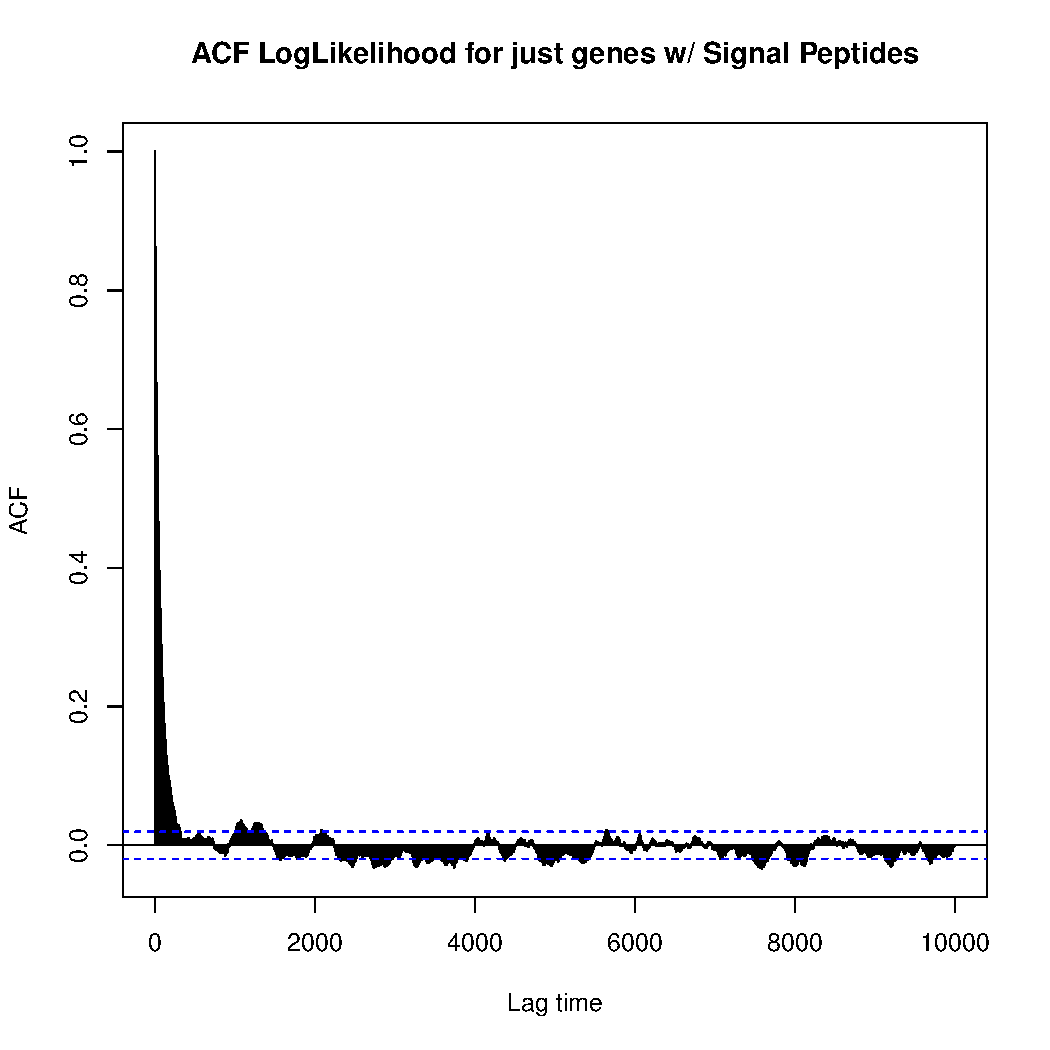
\includegraphics[page=1,scale =0.5]{Model_checking/acf_loglikelihood.pdf}}
\newline
$\bullet$ Started NSF Graduate Fellowship application.

\experiment{11-17-2016}

\subexperiment{Summary of work since last update}
October was mainly driven by NSF GRFP application, colloquium presentation for Grant Writing, and writing NSF-style proposal for Grant Writing class. Time dedicated to TAing for the LFSC 507 class has not been insignificant as I had to learn the Python packages NumPy, SciPy, and Pandas for some of my lectures. 
\newline
However, I was able to make significant progress on the Signal Peptide project (see section "Signal Peptide Project - Progress as of 11-17-2016" for details).
\newline \newline
Mike's comments regarding current results: \newline
$\bullet$ Overall, it seems like selection on CUB within signal peptide regions is in the same direction as the rest of the genome. However, there might be some differences in the strength of selection for certain codons. \newline \newline
$\bullet$ Standard linear regressions were used for generating the plots found in the Signal Peptide Project section. Weighted least squares regression would be a more valid approach due to the deterministic variables in these cases are not equally precise. I can modify the function I used to generate these plots to take in a boolean variable specifying whether or not the user wants to use ordinary or weighted least squares and perform the appropriate calculations. (Note: need to look into weighted least squares first). \newline \newline
$\bullet$ When treating $\Phi$ values as given and not estimating them, treated them as the true $\Phi$ value, ie. variation in $\Phi$ is 0. This is certainly not the case. A better approach might be to calculate the average standard deviation for each $\Phi$ from the different samples and use these to allow the genes to vary when estimating $\Delta\eta$. I will need to measure the autocorrelation of the $\Phi$ traces to make sure the samples are independent of the previous samples. \newline \newline
$\bullet$ Results for the signal peptides and first 31 codons in genes lacking a signal peptide (Figures 5a and 7a) seem more consistent with selection against nonsense errors in the 5' regions of the genes. To be more certain of this, instead of doing first 31 codons for all genes, can calculate mean and variance of signal peptide length and use these to draw cutoff points for splitting the genes. Signal peptide regions are generally 20 to 40 amino acids long. An alternative approach is take the first 20 codons,truncate out the next 20, and then take the the rest of the gene. \newline \newline
$\bullet$ Would be helpful if plots comparing $\Delta\eta$ values between mixtures generated by module plotParameterObject.R also included error bars. \newline \newline

Other current work:\newline
1) The plotModelObject.R module cannot generate the codon usage frequency plots (as function of $log\Phi$) when not estimating expression. I started fixing this on 11-16-2016. Part of the problem with the current implementation is it relies on making calculations from the last samples of the traces. When not estimating a parameter, the traces for that parameter are not updated, resulting in the traces being filled with the value 0. I'm modifying the code to initialize the $\Phi$ traces with the initial values provided by the user. If no values are provided, the traces will be initialized with 0.0, as they are now. The advantage of this is it allows us to handle this situation of not estimating parameters without requiring a bunch of if-else statements to the code.
\newline
2) In Bob's lab, I promised to assist Mallory Ladd with the data analysis for a project she is currently working on and will present at a conference in a few weeks (with the promise of being listed as a co-author on the project). This project involves looking at liquid chromatography tandem mass spectrometry (LC-MS/MS) measurements of metabolites in soil water samples. Metabolomics data is usually more complicated than proteomics data because of the greater variability in the chemical structures of metabolites relative to peptides. 
\newline
3) I need to finish modifying the current ribModel framework to treat $\Phi$ as a mixture of lognormal distributions. I need to implement the traces to keep track of the additional hyperparameters approximated by the model and actually test the code to make sure it works. \newline \newline

Other stuff: \newline
$\bullet$ Assisting older students in GST with their preliminary exam by providing feedback on proposals/presentations. This has given me some insight into the GST prelim process. The combination of this and Grant Writing should result in my own prelim going smoothly next year...hopefully. \newline
$\bullet$ Signed up for Outreach on Darwin Day website. I suggested last night at the meeting for Darwin Day that we consider doing something similar to "Pint of Science" which will allow general public to interact with scientists in a more informal context. I already harassed a couple of my closer friends in GST and they seem interested in helping out.
$\bullet$ Final draft of proposal for Grant Writing is due November 22nd by 5 pm, so I've been working on making some edits to that the past couple of days.
\newline
Plans for the coming month (ordered by my current priority):
1) Make improvements to statistical approach and plots based on Mike's suggestions. Bob has said he would also like me to look at signal peptides in \textit{C. thermocellum} and \textit{C. bescii}, but I expect we will find similar results to \textit{E. coli}. Given the relatively short time it takes to fit ROC to data, it wouldn't hurt to perform the additional runs.   
2) Assist Mallory with data analysis. Poster presentation is in a few weeks. We have exchanged a few papers regarding metabolomics and current data analysis tools. We are meeting tomorrow (11-18-2016) to discuss ideas.
3) Finally finish $\Phi$ mixture distribution. 


\experiment{11-18-2016}

\subexperiment{Meeting with Mallory}

Meeting to discuss analyzing data from LC-MS/MS runs on soil water data.

First step is defining metabolite features based on mass and retention time, but these are dependent on sample preparation and data acquisition (so like a hierarchical model). Choice of solvent, biological matrix, etc. can affect factors such as elution and chromatographic separation. Artifacts can be generated based on desorption and ionization processes. In summary, results are highly dependent on experimental parameters and sample preparation. [Yao \textit{et al}, Metabolites, 2015]
\newline

Mallory has a bunch of samples. Each file contains MS1 and MS2 scan info for top 10 most abundant in each MS1 scan. 

\experiment{12-7-2016}
Have been looking into linear errors in variable models. Have not been able to find much that makes immediate sense to me. However, there are two potential programs/packages I might be able to take advantage of. Leiv is a R package that came out a few years ago. Seems to take Bayesian approach. STATA also has some tools. UTK students have access to STATA through 


\subexperiment{Gilchrist lab meeting}
Phi is expression rate observed given current set of amino acids and psi is the expression at the optimal amino acids. Adjusted gene expression is psi/phi. So if you have psi of 1 and phi of 0.8, need to produce 20 percent more.

Read McCandlish papers Mike sent today.

E-score in BLAST means the likelihood of finding a match just by chance, the lower the better. 

Description of ROC paper...possibly help Cedric with paper and documentation

Get on the gene expression mixtures.  

Would probably be a good idea to take some more formal statistics classes in the next few years. I emailed Russ to ask if he knew any good courses to take. He recommended:

Math 525 and 526 or Stat 563 and 564. These are both series courses to be taken over the course of one academic year. He also recommended Stat 577, Data Mining. 

Added confidence intervals to module for plotting Parameter objects in RibModelFramework. Also have altered code to work make CUB plots even when not estimating expression. This fix was implemented by initializing traces with initial values if present. I want to test this a little bit more before I push anything to the repository. 

\experiment{12-8-2016}
Working on finishing up the mixtures of gene expression values. Found a typo in the code that caused R to not be able to see some of the functions for getting the $s_\phi$ trace. Code currently compiles and runs. 

Bob and I discussed last week about redoing the analysis for signal peptides only using genes predicted to have a signal peptide with a high D-score (>0.75). The D-score is a weighted average of other metrics approximated by SignalP. From my understanding, the closer the score is to 1.0, the better the prediction. My understanding of the details will require me to read the SignalP papers (probably for both versions 3.0 and 4.0). For \textit{E. coli}, there are 266 genes that fall into this category. 

Read up on some linear regression stuff. Signed up for some Coursera lectures on regression modeling, statistical inference, and genetics/evolutionary biology. My guess is these are geared more towards undergraduate, but they might have some information useful to me. I can have the lectures playing in the background while I work and if something should sound unfamiliar, I can pause my work to pay closer attention. Also read a little bit from \textit{The Elements of Statistical Learning}.

\experiment{12-12-2016}
Having issues implmenting gene expression mixture. Currently getting a segmentation fault. 


\experiment{12-14-2016}
\subexperiment{Gilchrist Lab Meeting}
SMA R package -> look into

HMM make inferences about shifts in optimal amino acids

Cedric will be taking over plotting $\phi$'s to Selac for empirical.

Meeting with Albrecht's lab at 3 pm. 

Make people do commits and pushes more often to GitHub

Github book that is free online. Software Carpentry might be worth looking into, also.

\subexperiment{Meeting with Albrecht and Ricardo}
Group from UK, mRNA levels in yeast, 600 transcripts oscillate over cell cycle fine resolution time. Use graph algorithm for studying biological networks

Thermodynamic analysis -> use chemistry concept to analyze networks
	- Entropy and information
	- Difficult to tell things from current analyses
	- We're interested because cyclical data, can methods be applied to 			  circadian rhythms
	 

Data collected is very descriptive in nature. Growth rate, meristems of root, translation regulation of genes involved in control of cell cycle. Periodic. Generate ribosome footprint data. Ribosome TRAP genetically label ribosome in certain cell types, pull down specific ribosomes from certain types. Express genetically modified ribosome proteins under certain tissue specific conditions.  

Albrecht has talked to the Pakanara's group about teasing out networks of translational efficiency (function of ribosomes per mRNA). Plenty of published data sets. Have not been analyzed comprehensively. 

Big questions:
1) When plants are exposed to two different conditions, some genes will be expressed similarly, some will be different. What does this tell us about signal transduction? Different conditions sometimes results in similar expression patterns. Why? 

Lack time series data at translation level, but might have it at transcriptional level. 

Signal transduction -> apply different stressors, do these affect different genes in the same way or not. One particular group (ribosomal proteins) of mRNAs respond to a wide-range of conditions can be target. These proteins are highly regulated at translation level. Ribosomal proteins appear to be co-regulated. If you look closely, you can convince yourself that these are actually different. Is this true? 

Mike proposes we think about current framework Ricardo is working with, and modify it to work with this project. Ratio of $\kappa$ to $\delta$. Tease out differeces between $\kappa$ and $\tau$. 


\experiment{12-15-2016}

Git tutorial:
1) Create new directory and while in the directory use git init command
2) Use git add <filename> to track changes to file(s)
3) Can use git status to check for changes
4) Can commit using git commit -m "<message>"
5) Can add remote repository with git remote add <remote name> <repository url>
6) Push to remote repository with git push -u <remote name> <branch name>. 
-u tells git to remember these parameters for later use, can just enter git push
7) git pull <remote name> <branch> to get changes from remote repository
8) git branch <branch name> to create a new branch
9) git checkout <branch name> to look at a new branch 
10) git merge <branch> to merge changes made in branch with current branch
11) can unstage a file using git reset <file name>
12) git checkout -- <file name> can be used to go back to last commit

\subexperiment{Student comments regarding LFSC 507}
$\bullet$ Need to provide more instructions for assignments.\newline
$\bullet$ Alex was a very good teacher, although it would have been nice to receive feedback on our labs a little more consistently. \newline
$\bullet$ Alex was very knowledgable and extremely helpful. He always responded promptly and granted extensions when they were needed by the students. His ability to keep his cool and act professionally even when certain individuals who were sitting in on the course were very rude was impressive. I would readily take another class that he was TA'ing for. \newline
$\bullet$ I really appreciated the quick responses and the help with the lab portion of the course - the labs were difficult but I felt like they really helped and that I was able to learn a lot from them. \newline
$\bullet$ I liked how accessible he was when needing help on the assignments. He had a good teach style for learning the material as easily as possible. \newline
$\bullet$ The workload was a lot, after the first couple of labs the time it took to complete them increased significantly. I really enjoyed the labs though, I learned a lot. \newline
$bullet$ Some of the later labs were quite long. It would be nice to get uploaded keys after the labs are due as well to be able to look over and see correct or better ways to do certain assignments. \newline
$\bullet$ I had no feedback for Alex specifically, I thought he did a great job. Although the class asked to learn some R, I thought time would've been better spent continuing with python. . This would allow students to go a bit further with the material. Finally, the older guy in the labs was extremely distracting, repeatedly heckling the TAs and should not be allowed to sit in on further courses. He actively took away instruction time and hindered the learning of students in the labs. I think he may be a biology instructor, and if this is the case, the department chair needs to have a serious discussion with him. His behavior was unprofessional and downright extremely rude and disrespectful to the other students and to the TAs. \newline
$\bullet$ I greatly enjoyed the python section, and I recommend that the course be turned away from fortran (a language I can't see myself using in my research) and more towards python. \newline



\experiment{1-6-2017}
Took a set of genes not predicted to have signal peptides and treated them as pseudo-signal peptides genes. The psuedo-signal peptide region was the first 23 codons, which is the average length of a signal peptide in \textit{E. coli}. This set of pseudo-signal peptides was chosen such that the average expression and standard deviation would be appoximately equal to those of genes with signal peptides (0.95 and 0.42, respectively). The comparison of $\Delta\eta$ estimates from a ROC fitting treating the pseudo-signal peptides and pseudo-mature peptides as separate categories is shown below in Figure 1. It is worth noting that this is a better correlation than the $\Delta\eta$ seen between actual signal and mature peptides.



Wanted to check to makes sure $\Delta\mathit{M}$ values were correlated between the different categories. Results can be seen in Figures 2-5. Figures 2 shows that $\Delta\mathit{M}$ estimates for non-signal peptides genes are approximately equal when fit with either mature peptides or signal peptides as a separate cateogory. $\Delta\mathit{M}$ is shared in these runs, this implies a strong correlation between these estimates for signal peptides and mature peptides, which can be seen in Figure 3. It is worth noting that estimates of $\Delta\mathit{M}$ for mature peptides across model fittings do not have the approximately $y = x$ relationship we would like to see (Figure 4). The same is true for signal peptides (Figure 5). Part of this could be because when the mature peptides or signal peptides are fit along with non-signal peptide genes, expression is estimated. However, when mature peptides and signal peptides are fit in the same run, expression is treated as absolute and not estimated. This likely affects the estimates of $\Delta\mathit{M}$.

\begin{figure}[H]
\fbox{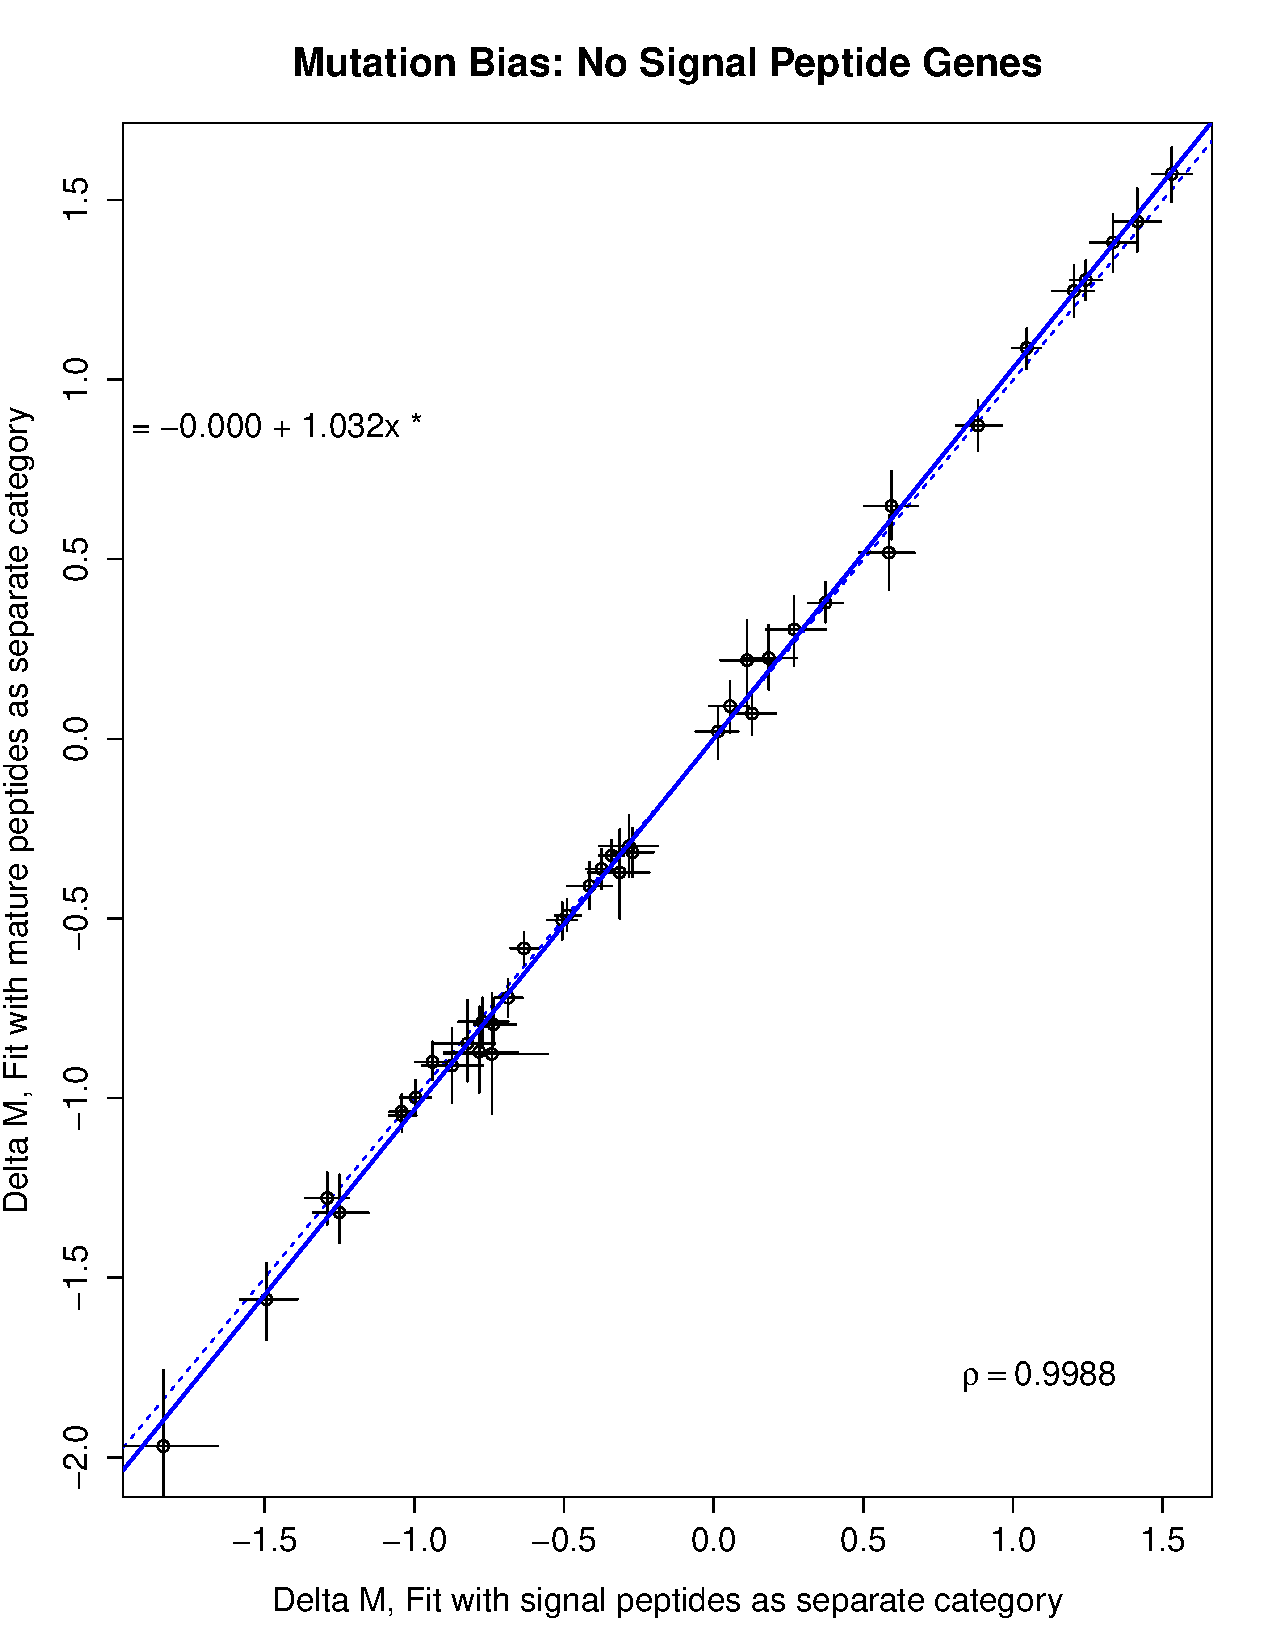
\includegraphics[page=1,scale=0.5]{Ecoli_results/Mutation_comparisons/Comparison_delta_m_nosp_categories.pdf}}
\caption{Comparison of $\Delta\mathit{M}$ values of genes not containing signal peptides (NoSP). The x-axis represents the $\Delta\mathit{M}$ values when NoSP is fit with signal peptides treated as a separate category. The y-axis represents when $\Delta\mathit{M}$ values when NoSP is fit with mature peptides treated as a separate category.}
\end{figure}

\begin{figure}[H]
\fbox{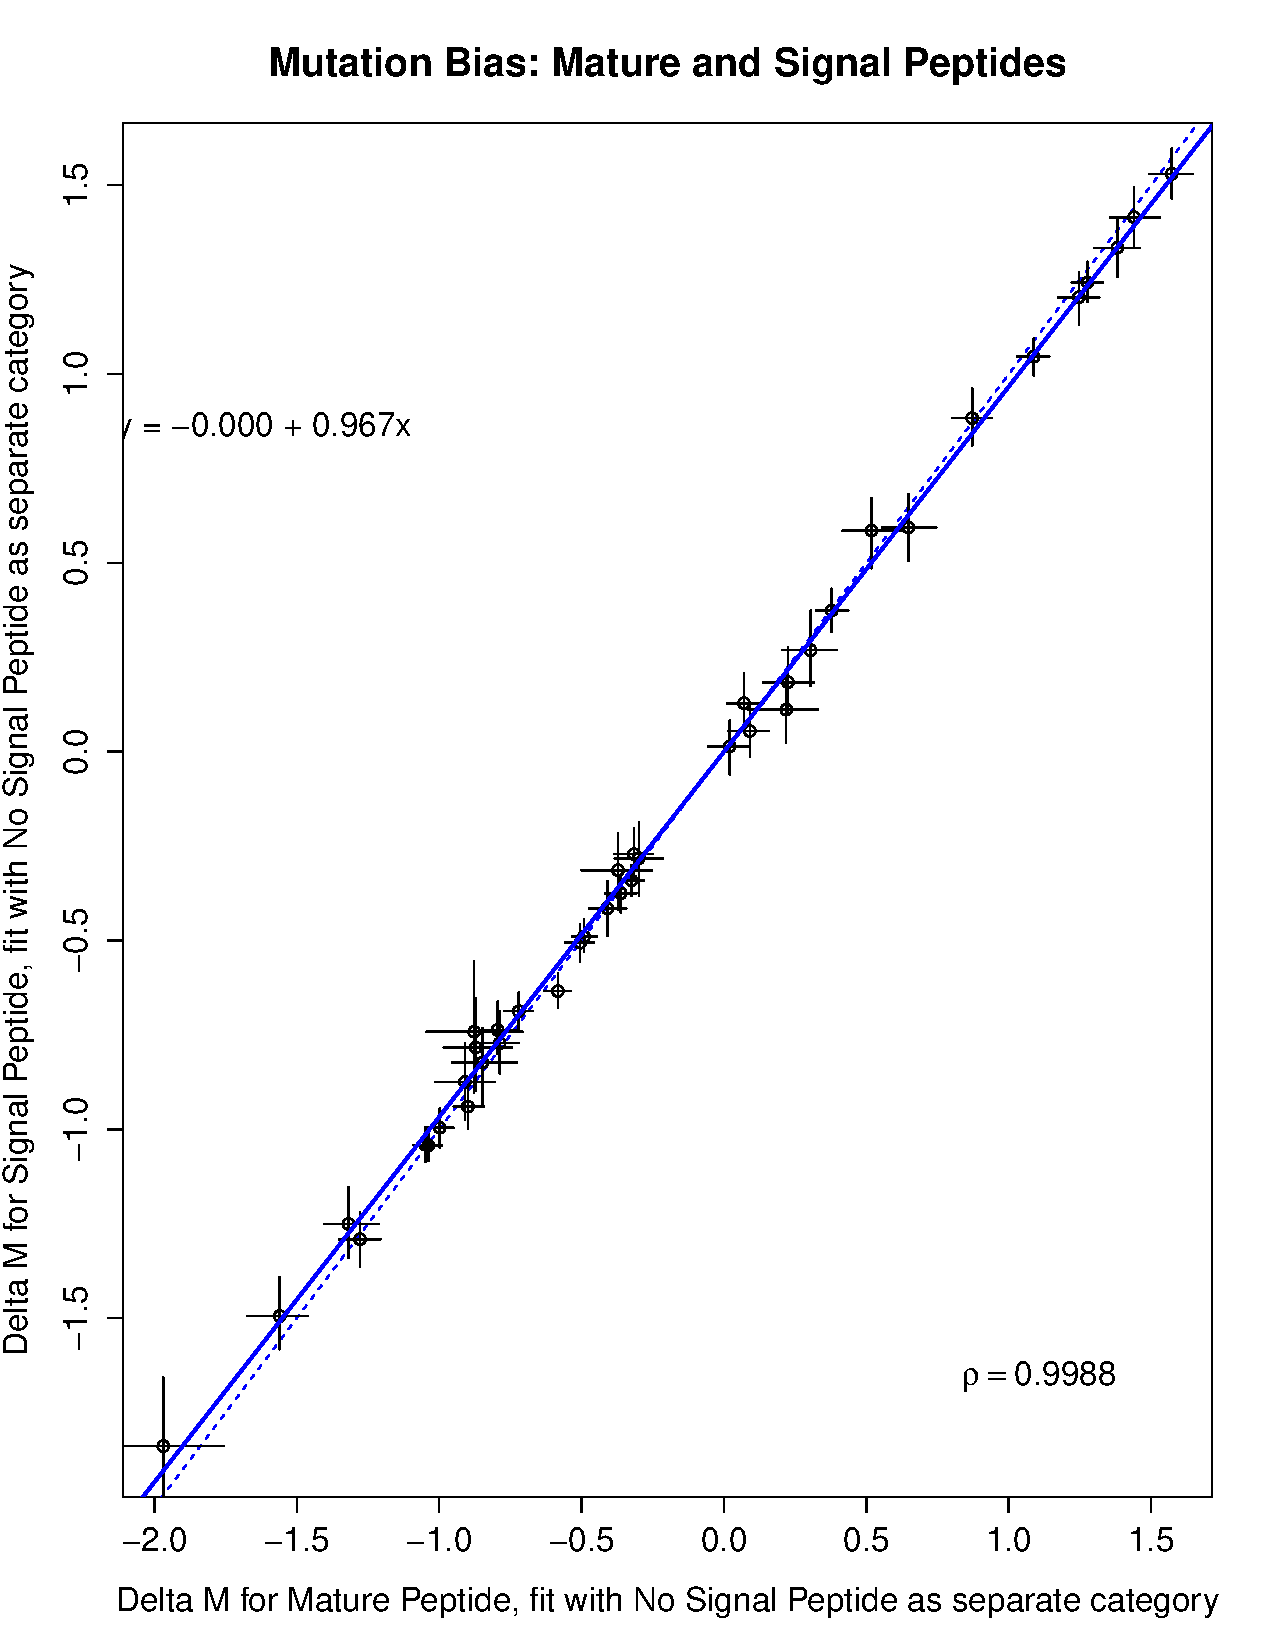
\includegraphics[page=1,scale=0.5]{Ecoli_results/Mutation_comparisons/Comparison_delta_m_sp_mp_when_nosp_separate_category.pdf}}
\caption{Comparison of $\Delta\mathit{M}$ values of signal peptides (SP) and mature peptides (MP), both fit with genes with no signal peptides as a separate category. The x-axis represents the $\Delta\mathit{M}$ values of SP. The y-axis represents when $\Delta\mathit{M}$ values of MP.}
\end{figure}

\begin{figure}[H]
\fbox{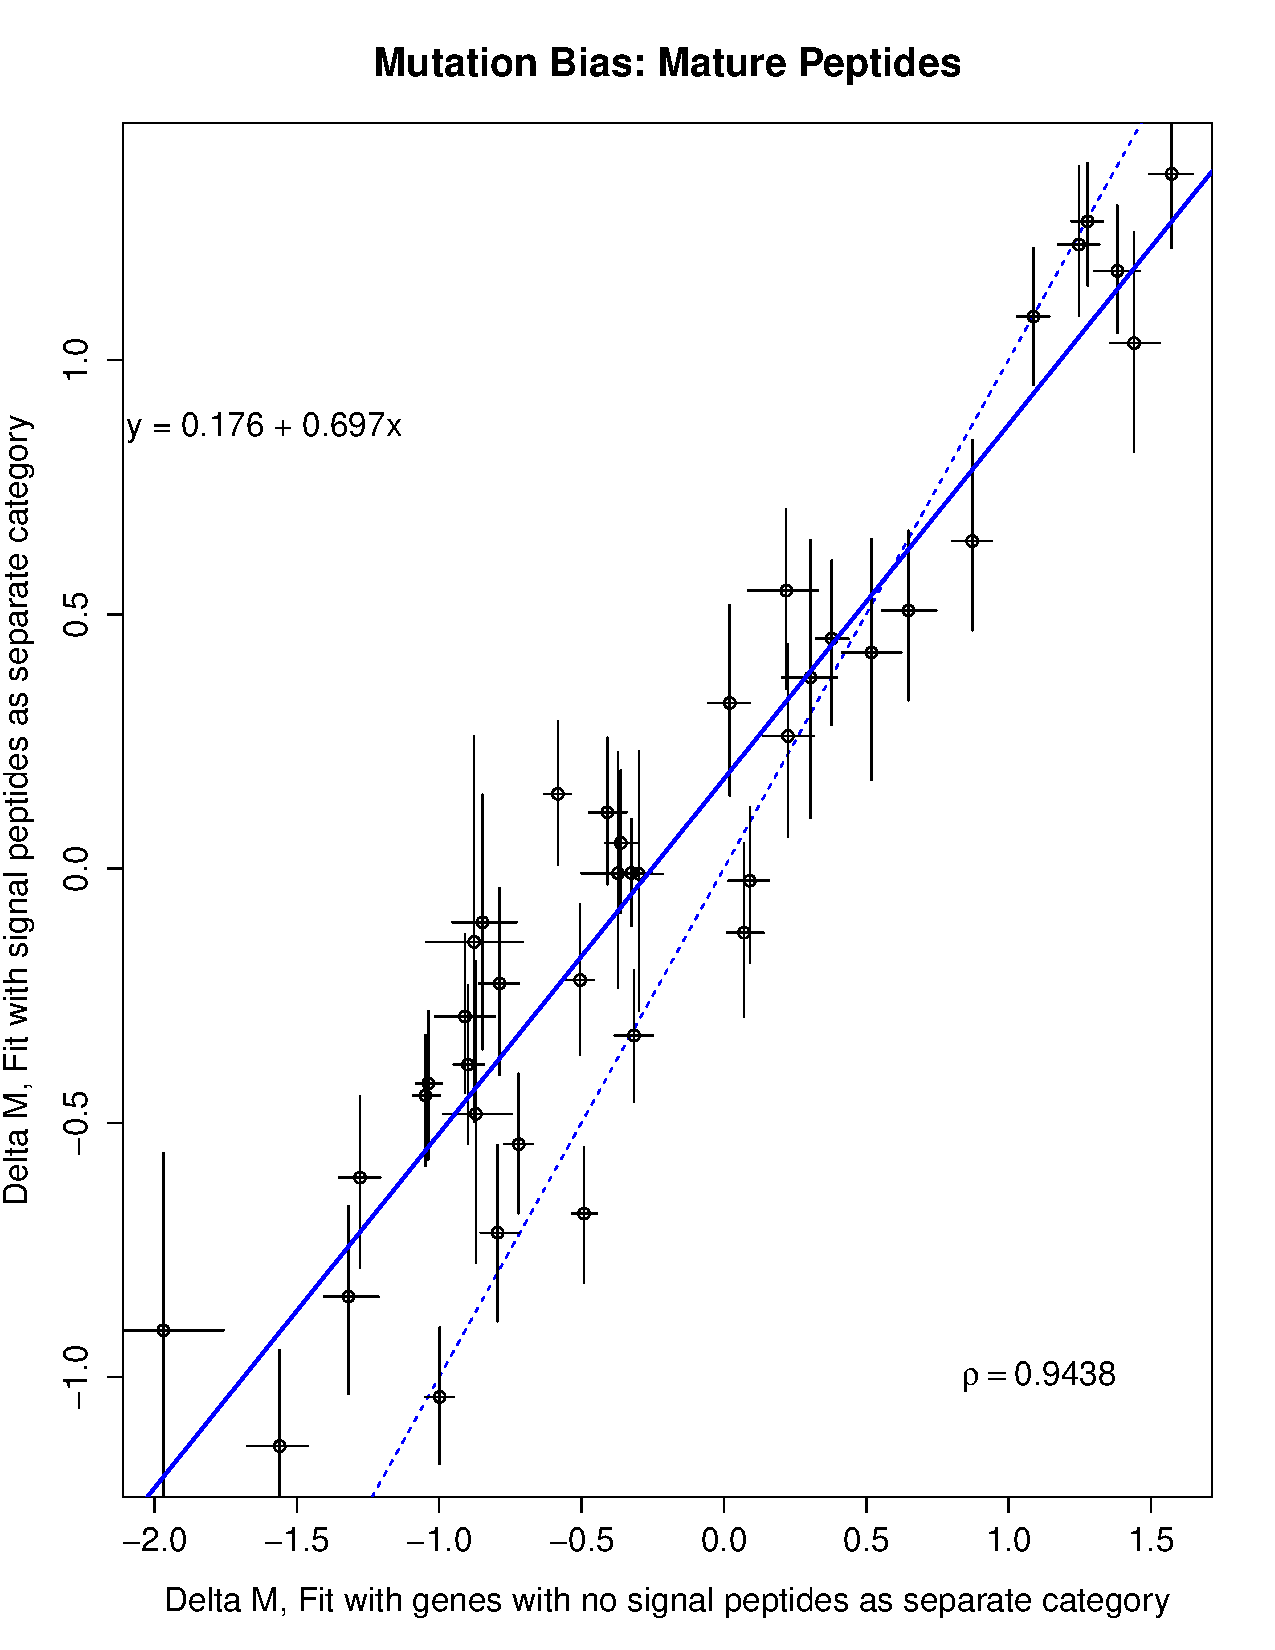
\includegraphics[page=1,scale=0.5]{Ecoli_results/Mutation_comparisons/Comparison_delta_m_mp.pdf}}
\caption{Comparison of $\Delta\mathit{M}$ values of mature peptides (MP). The x-axis represents the $\Delta\mathit{M}$ values of MP when genes with no signal peptide is treated as a separate category. The y-axis represents the $\Delta\mathit{M}$ values of MP when signal peptides are treated as separate category. In the latter case, $\phi$ is not estimated, but treated as constant. This might explain why the $\Delta\mathit{M}$ values deviate from the y=x line.}
\end{figure}

\begin{figure}[H]
\fbox{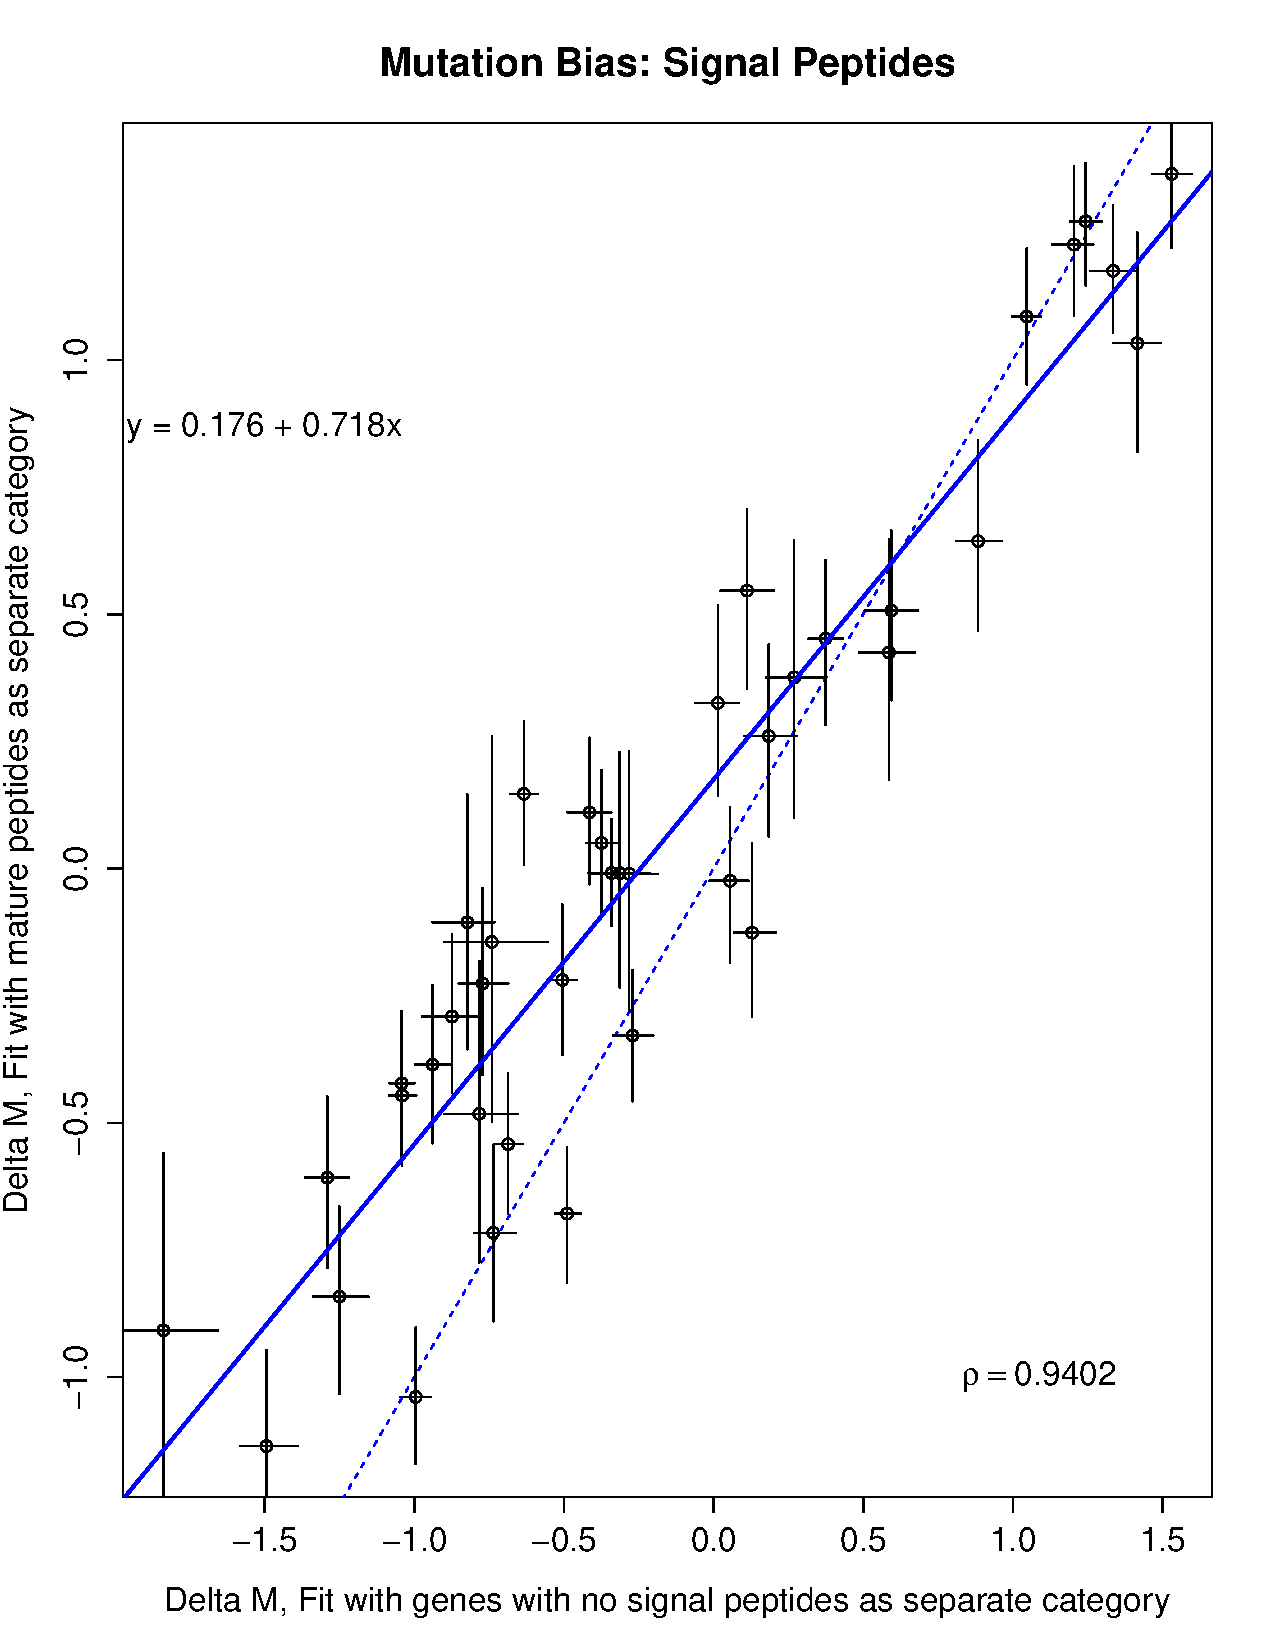
\includegraphics[page=1,scale=0.5]{Ecoli_results/Mutation_comparisons/Comparison_delta_m_sp.pdf}}
\caption{Comparison of $\Delta\mathit{M}$ values of signal peptides (SP). The x-axis represents the $\Delta\mathit{M}$ values of SP when genes with no signal peptide is treated as a separate category. The y-axis represents the $\Delta\mathit{M}$ values of SP when mignal peptides are treated as separate category. In the latter case, $\phi$ is not estimated, but treated as constant. This might explain why the $\Delta\mathit{M}$ values deviate from the y=x line.}
\end{figure}


Over break, collected data for \textit{C. bescii} as a comparison to the results in \textit{E. coli}. Signal peptides in \textit{C. bescii} showed similar behavior to those in \textit{E. coli}. Below is a comparison of the $\Delta\eta$ values for signal peptides and mature peptides in \textit{C. bescii}. Much like in \textit{E. coli}, selection is generally in the same direction, meaning highly selected for codons in one region are likely to be highly selected for in the mature peptides. It should be noted that in the signal peptide regions, the arginine codon CGG trace appears to trend towards inifinity. As a result, this one is excluded from many of the plots. 

\begin{figure}[H]
\fbox{\includegraphics[page=2,scale=0.5]{Cbescii_results/Nosp_w_mp_cat/Graphs/cbescii_dEta_dM_comp_plots.pdf}}
\caption{Comparison of $\Delta\eta$ values of genes with no signal peptides and mature peptides.}
\end{figure}

\begin{figure}[H]
\fbox{\includegraphics[page=2,scale=0.5]{Cbescii_results/Nosp_w_sp_cat/Graphs/cbescii_dEta_dM_comp_plots.pdf}}
\caption{Comparison of $\Delta\eta$ values of genes with no signal peptides and signal peptides.}
\end{figure}

\begin{figure}[H]
\fbox{\includegraphics[page=6,scale=0.6]{Cbescii_results/Nosp_w_sp_cat/Graphs/cbescii_nosp_w_sp_cat_traces.pdf}}
\caption{Traces of $\Delta\eta$ values for signal peptides when fit with genes with no signal peptides as a separate category. Many of the traces do not look like they are mixing well. Also, the arginine codon (R) CGG looks unrealistically high. This may need to be run for more iterations.}
\end{figure}

\begin{figure}[H]
\fbox{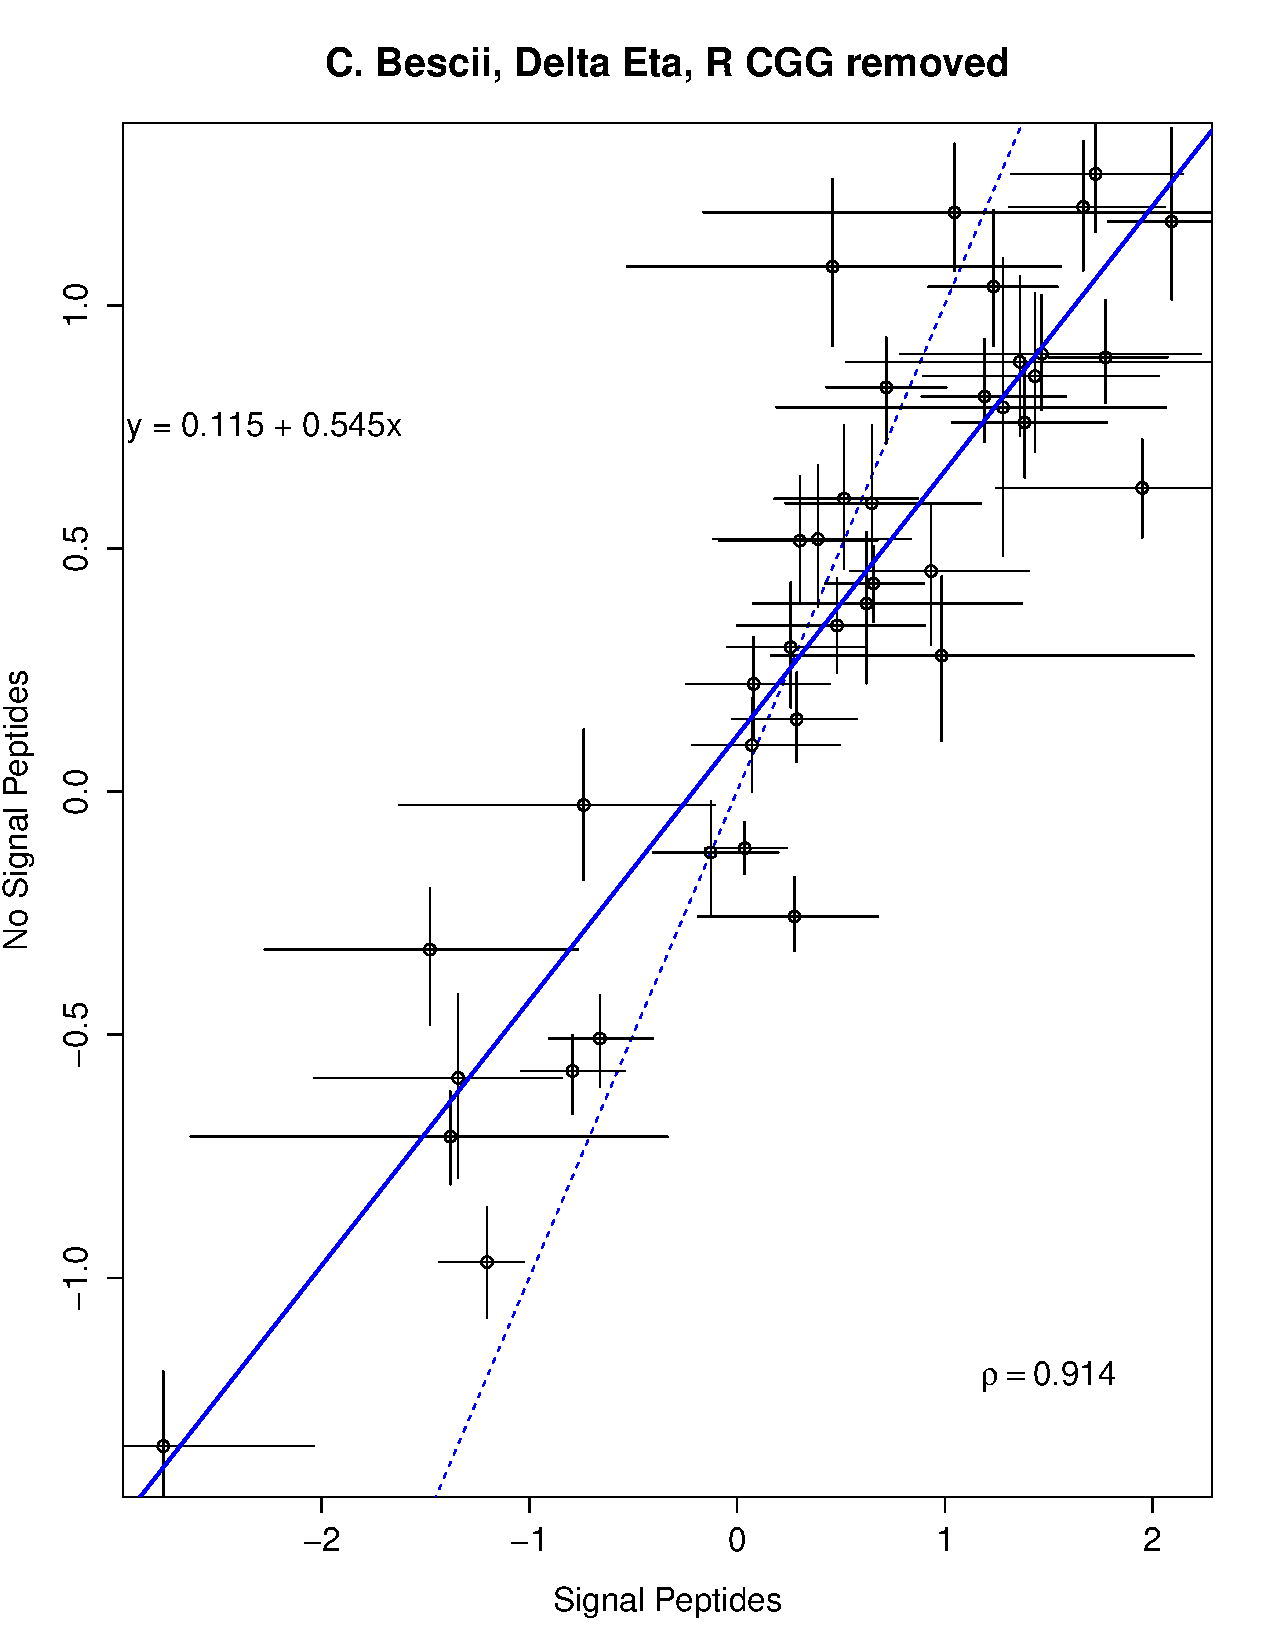
\includegraphics[page=1,scale=0.5]{Cbescii_results/Nosp_w_sp_cat/Graphs/delta_eta_comp_R_CGG_removed.pdf}}
\caption{Comparison of $\Delta\eta$ values of genes with no signal peptides and signal peptides. Same as Figure 6, but arginine codon CGG removed.}
\end{figure}


\experiment{1-10-2017}
\subexperiment{$\phi$ Mixture Model}
Tested mixture model for $\phi$ using \textit{S. cerevisiae} genome taken from \underline{yeastgenome.org}. Results of traces and CUB plot shown in Figures 10 - 12. Traces of Log(Posterior Probability) and expected value of $\phi$ shown in Figures 13 and 14. It is worth noting these results were taken with 100000 samples with 100 thining and 100 adaptiveWidth

\begin{figure}[H]
\centering
\includegraphics[page=1,scale=0.6]{Mixture_model_testing/Test_mixture/real_data/Graphs/yeast_deltaEta_deltaM_traces_CUB_plot_updated.pdf}
\caption{$\Delta\mathit{M}$ traces with mixture model for $\phi$}
\end{figure}

\begin{figure}[H]
\centering
\includegraphics[page=2,scale=0.6]{Mixture_model_testing/Test_mixture/real_data/Graphs/yeast_deltaEta_deltaM_traces_CUB_plot_updated.pdf}
\caption{$\Delta\eta$ traces with mixture model for $\phi$}
\end{figure}

\begin{figure}[H]
\centering
\includegraphics[page=3,scale=0.6]{Mixture_model_testing/Test_mixture/real_data/Graphs/yeast_deltaEta_deltaM_traces_CUB_plot_updated.pdf}
\caption{CUB plot with mixture model for $\phi$}
\end{figure}

\begin{figure}[H]
\centering
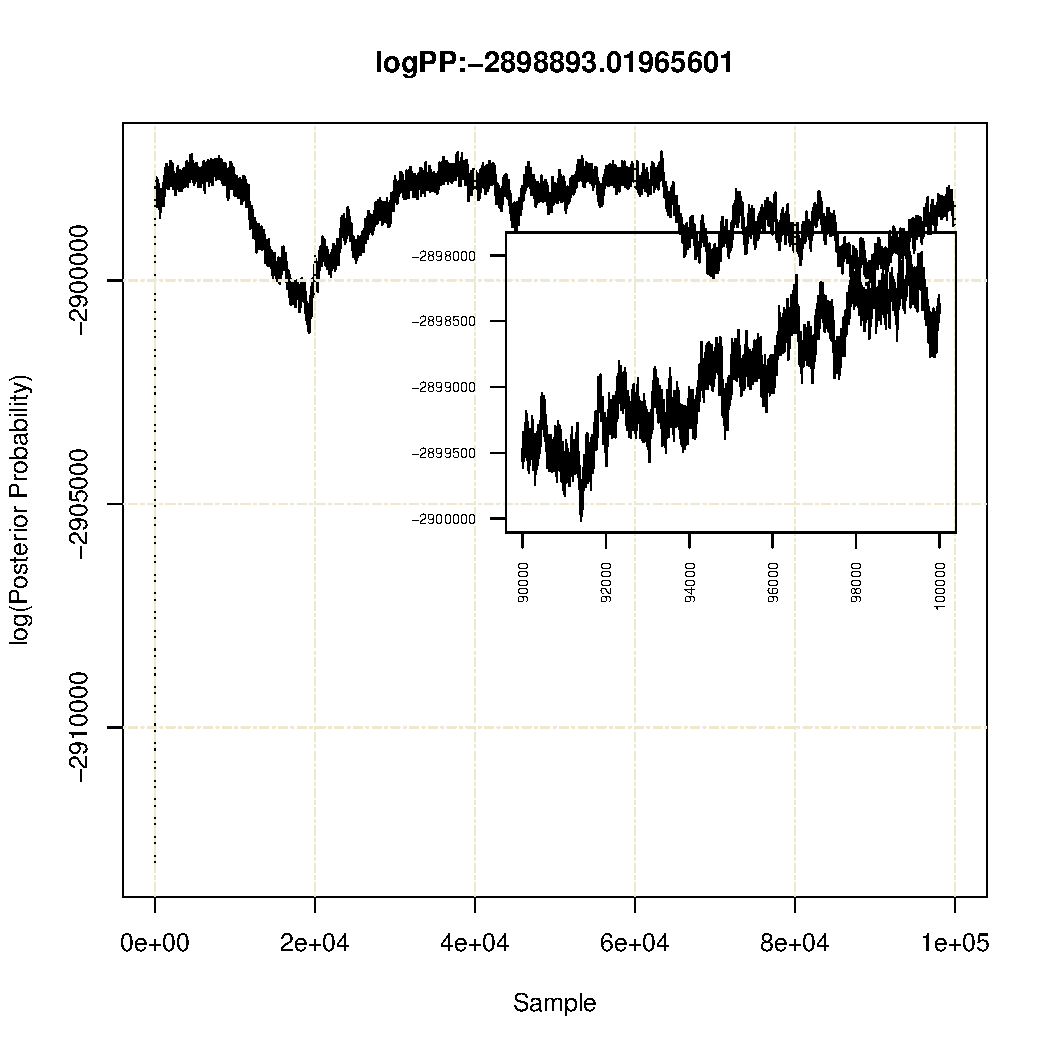
\includegraphics[page=1,scale=0.6]{Mixture_model_testing/Test_mixture/real_data/Graphs/yeast_logPost_mixProb_phi_traces_updated.pdf}
\caption{Log(Posterior Probability) trace with mixture model for $\phi$}
\end{figure}

\begin{figure}[H]
\centering
\includegraphics[page=9,scale=0.6]{Mixture_model_testing/Test_mixture/real_data/Graphs/yeast_logPost_mixProb_phi_traces_updated.pdf}
\caption{Expected value of $\phi$ trace with mixture model for $\phi$}
\end{figure}


\experiment{1-11-2017}
\textit{Meeting with Mike}
Likelihood ratio tests for treating them as same categories vs together. \textbf{Question: From a statisical philosophy point of view, can you take parameters estiamted in a Bayesian context and apply Frequentists/Classical hypothesis testing?} Fit model to mature peptides + pseudo-mature peptides. Compare confidence intervals. See if they overlap. Look up Deviance Information Criterion, might be useful here. Do the same thing for pseudo-signal peptides. 

Redo runs from before, but let diverge for about 100 iterations. Do traces converge to same spot. This gives confidence that our parameter estimation is correct.

Add function for calculating autocorrelation for different traces to package.

\textit{C. bescii} looks like it hasn't converged, so just run for longer. \textbf{It's interesting to me that $\Delta\eta$ and $\Delta\mathit{M}$ values for \textit{C. bescii} seem to be struggling to converge, where as \textit{E. coli} seems to have no problems. These are both prokaryotic organisms. Why would they be so different?} 

\subexperiment{Plan Going Forward}


\experiment{1-16-2017}
Re-ran ROC treating non-signal peptide genes and mature peptides as separate regions, but this time MCMC was allowed to diverge for 100 steps. Comparisons of $\Delta\eta$ values can be seen below. Clearly, the divergence had almost no impact on the parameter estimates, giving confidence that these results are likely correct. 

\begin{figure}[H]
\centering
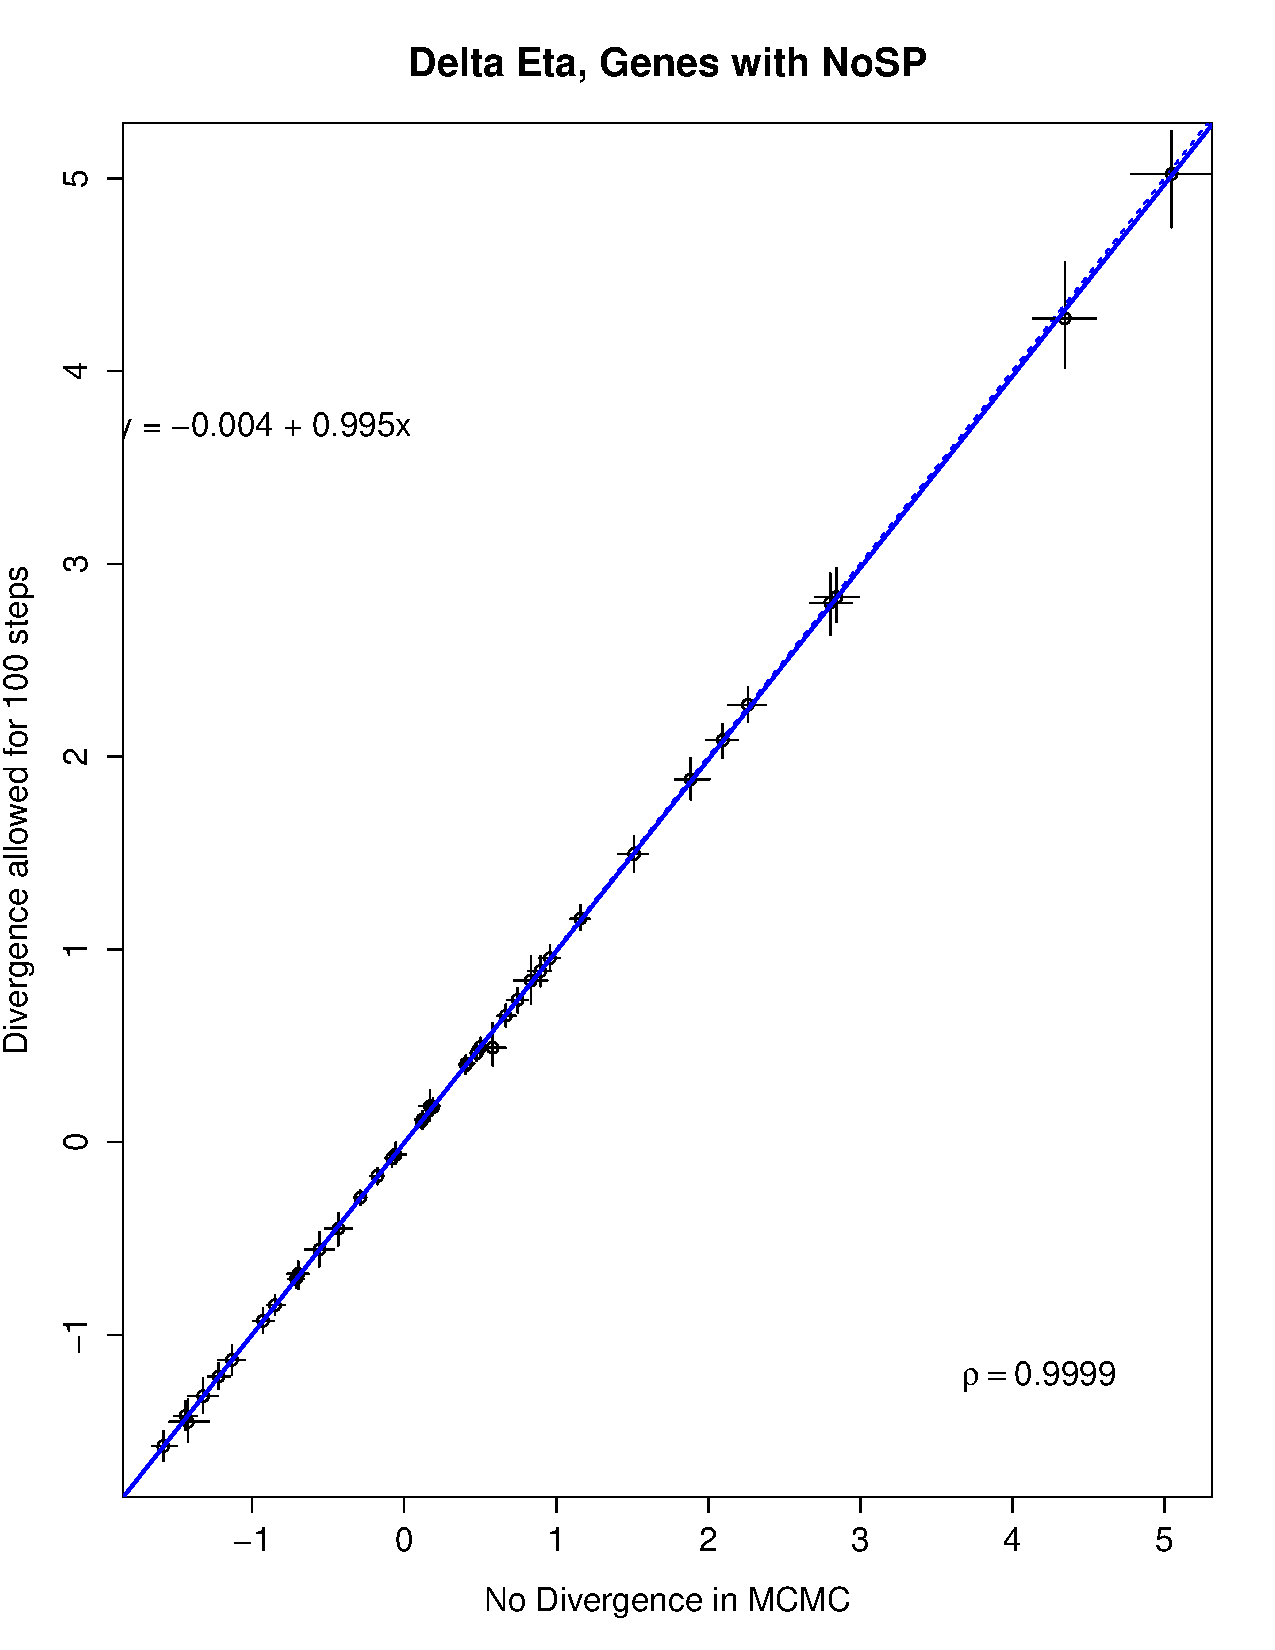
\includegraphics[page=1,scale=0.6]{Ecoli_results/Nosp_w_mp_cat_divergence_100/Graphs/Comp_nosp_no_divergence_to_divergence_100.pdf}
\caption{Comparison of $\Delta\eta$ estimates in non-signal peptides genes when MCMC not allowed to diverge vs allowed to diverge for 100 steps}
\end{figure}

\begin{figure}[H]
\centering
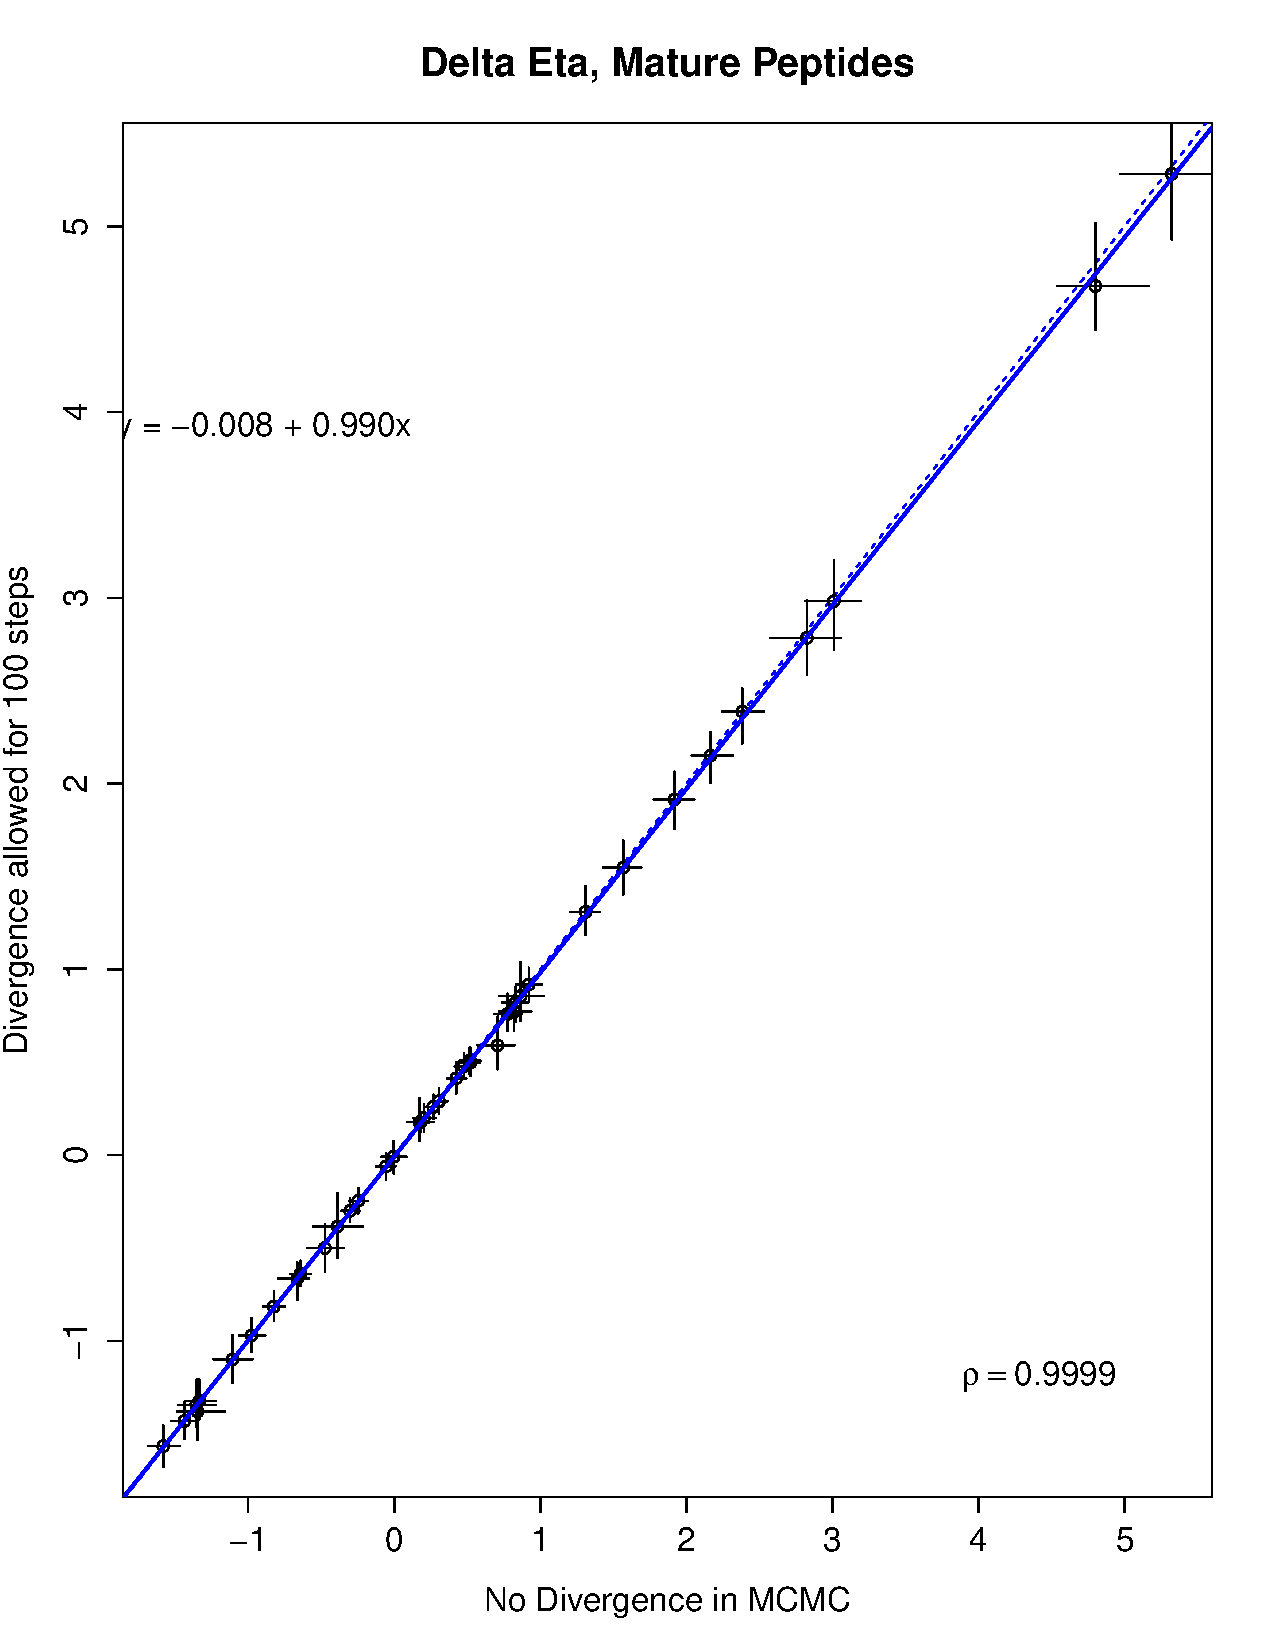
\includegraphics[page=1,scale=0.6]{Ecoli_results/Nosp_w_mp_cat_divergence_100/Graphs/Comp_mp_no_divergence_to_divergence_100.pdf}
\caption{Comparison of $\Delta\eta$ estimates in mature peptide regions when MCMC not allowed to diverge vs allowed to diverge for 100 steps}
\end{figure}

\experiment{1-18-2016}
Ran pseudo-mature peptides with actual mature peptides as separate categories. 



\textit{Meeting with Mike}
1) Make divergence more robust, if it puts you in realm of underflow or overflow, either go back a step and stop (produce warining) or step back and keep proposing something until numerically valid range. \newline
2) Find reference for rejection sampling, look back at Wikipedia sources \newline
3) Work on wrapping head around model comparisons \newline
4) Compare posteriors when treating sp and mp as the same thing \newline
5) Compare yeast to benchmarks, should be in testing \newline
6) Don't worry about initial conditions being worried about single lognormal distribution \newline
7) Fit mixture model to real data, simulate based on true value, fit to simulated data, do not expect much divergence. Then try with old approach. Expect values to climb. \newline
8) How do confidence intervals for signal peptides and pseudo - signal peptides overlap? \newline


\experiment{1-25-2017}
Reference for rejection sampling: "Generalized Accept–Reject sampling schemes", Casella et al, Institute of Mathematical Statistics Lecture Notes, Monograph Series \newline

Performed Likelihood Ratio tests for Mature Peptide and Signal Peptide, which indicated significance at significance level 0.005 (critical value 66.7659). However, this is also true of Non-signal peptide genes treating mature peptides as same or separate category (290). Ran only non-signal peptide genes, split into two cateogories of equal size, and compared this to previous run treating non-signal peptide genes as one cateogry using Likelihood ratio test. This again indicates significance (180). \newline
 
Compared yeast. Need to simulate genome, run with model.

\subexperiment{Lab meeting}
Cedric is trying to get at idea where C Left originated. Basd estimates off of Rocus tree. 

Calculate effective sample size (ESS), Coda in R. Look into ESS. Want around 500 for every parameter. Start with CSP parameter. After that what are ESS for acf. 

Take over autocorrelation stuff. Say thinning is 10. Run for longer, how do confidence intervals change? Do they grow? 

\subexperiment{Math Eco Seminar - Preface and Chapter 1}
The "best" model is constrained by the types of models you are considering. 

 
 
For acf, for phis, calculate average and std pf autocorrelations and plot these. Cedric saw some autocorrelation of the autocorrelation. How well does posterior probability trace autocorrelation reflect autocorrelation with other parameters (genome and CSP parameters). Alternatively, look at effetive samples sizes for the different parameters. 

\experiment{2-1-2017}
Autocorrelation

Effective sample size for posterior trace using Ecoli full genome, 5000 samples, 50 thinning, was roughly 35. 

Average effective sample size of phi traces 

Make sure burn-in is thrown out, add 95\% confidence intervals.


For acf, modify acceptance-rejection target, lower rate, expect greater independence. Possibly add code to stop after achieving some level of ESS. Also could start independent chains, let diverge, do they converge to the same value. 

Brian says not to change acceptance-rejection target, probably won't change much.


Looked at DIC for Mature peptides and Signal Peptides, and Pseudo Signal Peptides and Real Signal Peptides.

DIC for MP = SP: 269364.2
DIC for MP != SP: 268584.8

DIC for PSP = RSP: 88066.73
DIC for PSP != RSP: 87887.16

In both cases, DIC is lower for alternative model. However, DIC tends to favor models that are overfitting.

Ando (2007) notes some problems with DIC. It is assumed that parameteric family of probability distributions that generate future observations encompasses the true model, which is not actually the case. Observed data are used to both construct posterior distribution and to computer the posterion mean of expected loglikelihood, which results in underestimating the bias. Same data used twice in calculating number of effective parameters.

Ando proposed BPIC

Do 100K run for phi mixture model. Look at simulated genome. Take last half of current parameter traces.


\experiment{2-2-2017}
Began phi mixture run using 100000 samples for yeast. Also started 40000 sample run for E. coli for purposes of looking at effective sample size (ideally want around 500 samples for everything). Tried to further understanding of PBIC, but still not quite sure how to implement. Finished reading Chapter 3A for seminar presentation. Got first draft of ASMS abstract to Bob. Want to have submitted before 5 tomorrow.

\experiment{2-3-2017}
Large portion of day was spent editing the ASMS abstract. Bob really wanted me to include results for C. bescii and C. thermocellum, but I'm still not convinced about the reliability of these results. We spun this so that validation of the results is on-going. Talked with Suresh about getting some gene expression data for C. bescii, but he says the results have still not been processed and likely won't be useable at the moment. I found some C therm RNASeq results produced by the Steve Brown lab at ORNL, but it looks like these use different identifiers. Will need to find mapping.

I remembered today that I need to re-run some of the E. coli fittings with divergence. Cedric said he usually allows divergence for 10 iterations. 


\experiment{2-5-2017}
Spent part of today cleaning up and testing some code (stuff for ACF I wrote that will be added to the repository. Looks like I need to fix the $S_\phi$, $\epsilon$, $M_\phi$ hyperparameter plots for the  $\phi$ mixtures. Also need to update reading and writing restart files and Robjects to account for changes in code (such as save likelihood, etc.)

\experiment{2-6-2017} 
Got around to looking at results of E.coli fittings with divergence. Patterns for $\Delta Eta$ correlated well, but the slope deviated significanlty from 1 (roughly 0.5). This was certainly concerning and I began digging into the code in order to find out what was going on. I had previously allowed divergence for 100 iterations when fitting the non-signal peptide genes and mature peptides, but this did not result in the strange behavior I was currently seeing. I checked some of the previous updates to ROC to make sure none of the changes would cause these strange results Eventually, I realized the problem was in the varyInitialConditions() function in MCMCAlgorithm module. This function varies everything, even parameters not being estimated. This would be problematic in the cases where I do not estimate phi, such as runs where I fit to the mature peptides and signal peptides. By allowing the $\phi$s to diverge, I'm effecitively shifting the search space for the algorithm and it has no chance to get back to that space because $\phi$s will not be changed after the initial divergence. 

\experiment{2-7-2017}
Spent most of the day preparing for Math Eco seminar. Also assisted with Darwin Day. Tried simulating Yeast genome, but I got an error when I tried to load the saved parameter object. I will need to fix this before I can proceed further. Need to fix restart files and R objects issues before I proceed further. This will save me time in the future.  
 
\experiment{2-8-2017}
Realized I made a mistake in changing varying initial conditions. Somehow, I accidentally deleted the for loop in this function, so I need to redo the runs I did previously; however, I expect results should still be consistent with results that don't allow divergence. 

\subexperiment{Gilchrist Lab Meeting} 
Run DIC calculations on PseudoMp-Mp runs. 


\experiment{2-9-2017}
Made edits to Bioinformatics paper based on Mike's comments. Pushed to directory

\experiment{2-10-2017}
New functions for plotting posterior and likelihood seem to be working. Need to test on case where don't estimate expression. Will not modify code to update these terms when estimating hyperparameters. Seems unlikely there would ever be a case when someone wants just these parameters and to keep everything else constant. 

\experiment{2-12-2017}
Was testing something with my old implementation of the $\phi$ mixture model to make sure the hyperparameters were being updated. Noticed both epsilon terms were staying at 0. This might partially explain why results from that second run looked decent.



\experiment{2-13-2017}
\subexperiment{$\phi$ Mixture Model Math Notes}

Want to be able to represent $\phi$ estimates as mixture of two distributions to more accurately reflect empirical data. Typically, gene expression data appears bimodal, with the a distribution 


\experiment{2-20-2017}
\subexperiment{Meeting with Bob}

SIPROS - home built version of MiriMatch, allows for isotopic labeling 

We know the Adams and Kelly groups, so we can contact them if necessary. 


\experiment{2-22-2017}

I've been thinking about the divergence problem for MCMC. Goal was to make it if overflow or underflow occurred while diverging, then go back to the previous state and re-sample the parameters. This would be easy enough if dealing with unsigned or signed integers. If unsigned, the output is defined in C++. Signed integer arithmetic is not well-defined, but typically overflow will result in two positive numbers summing to produce a smaller number and underflow will result in two negative numbers summing for a positive. This would be very easy to detect. The problem is we are dealing with floats/doubles. The way these are defined by IEEE allows for gradual overflow or underflow. What this means is overflow/underflow will not occur the moment you 


\experiment{2-27-2017}
Make plots of phis for each segment - how do they vary
Plot uncertainty for all of the fits through the origin
Maybe can just initialize value and not estimate hyperparameters. Also reduce $s_\epsilon$ by an order of magnitude. 

Plot estimates of slope and intercept, how do they vary? We want to be able to tell if slope differentiates from 1 and if intercept differentiates from 0. How do confidence intervals vary from 1 and 0 (plot these lines, do they overlap). 

For Ctherm, check ribosomal genes are. Ideally, indicate where they are in CUB-expression plot histogram
Create histrograms of deltaEta and deltaM, grouped by third nucleotide for 2 codon amino acids only.  

Plot histogram of differences for delta etas. 

Start looking at journals for signal peptide paper for E.coli.  

\experiment{3-7-2017}
Potential journals for signal peptide paper
\begin{itemize}
	\item Biochemical and Biophysical Research Communications
	\item Nucleic Acids Research
	\item Trends in Microbiology
	\item BMC Genomics
\end{itemize}

\experiment{3-8-2017}

\textbf{Documentation to edit for ribModel package}
\begin{itemize}
	\item convergence\_test.Rd
\end{itemize}


\experiment{3-14-2017}

\subexperiment{Histogram of Phis by segment for \textit{E. coli}}
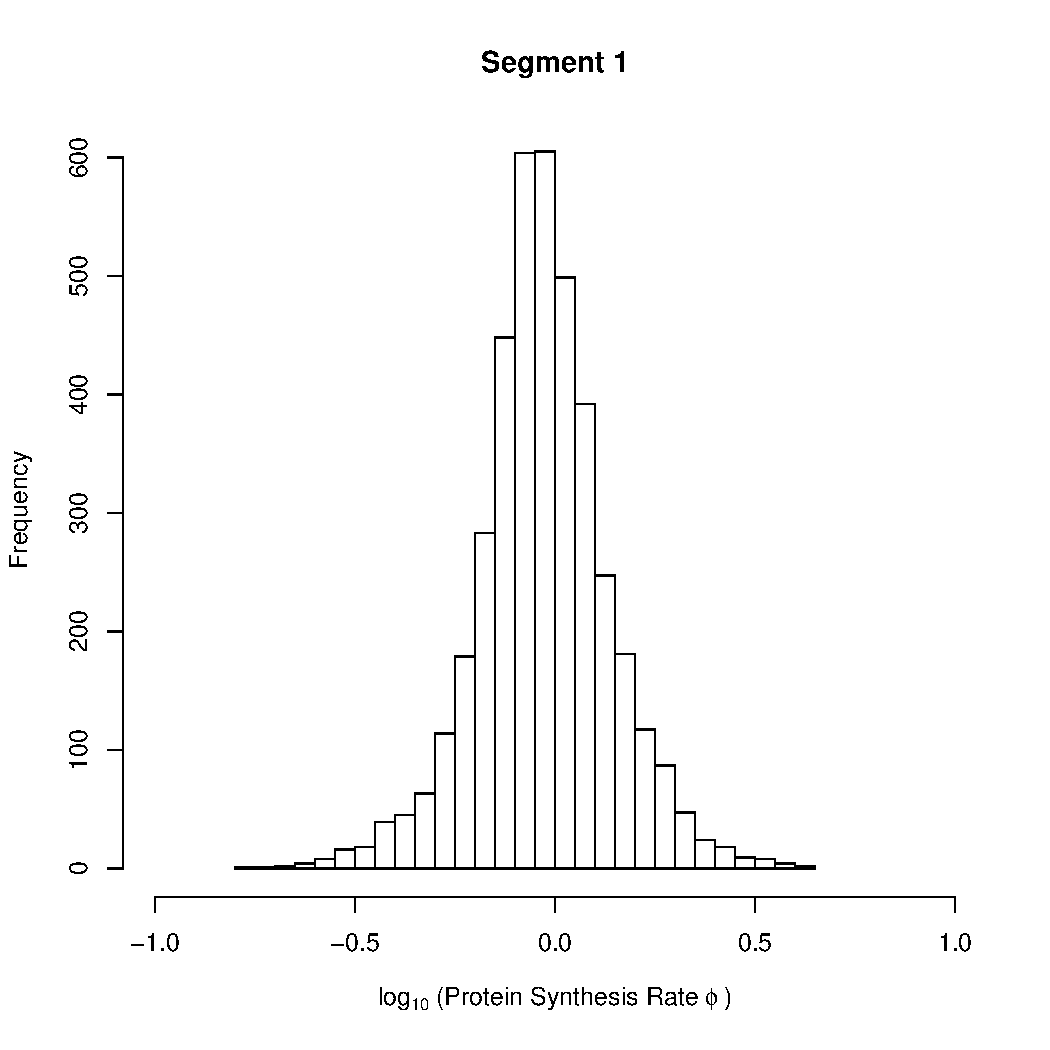
\includepdf[pages=-]{Ecoli_results/Segments_expression/Histograms_phis_by_segment.pdf}

\subexperiment{Histograms of $\Delta\eta$ and $\Delta\mathit{M}$ for \textit{C. thermocellum} 2 codon amino acids, grouped by 3rd codon}
\includepdf[pages=-]{Ctherm_results/Full_genome/second_run/Graphs/dEta_dM_histograms_2_codon_aa.pdf}


\subexperiment{Ribosomal Proteins for \textit{C. thermocellum}}
Bars marked with red means at least one ribosomal protein was contained in this range. Black or green mean a ribosomal protein was not found.

\includepdf{Ctherm_results/Full_genome/second_run/Graphs/ribo_prot_ctherm_dist.pdf}

\subexperiment{MLE search for linear regression when errors in both variables}

\begin{algorithmic}
	\State $iterations \gets 1000000$
	\State $start \gets 0$
	\State $end \gets 2$
	\State $step \gets 0.01$
	\State $\beta \gets start$
	\State $best.\beta \gets \beta$
	\State $likelihood.max \gets -\infty$
	\While {$\beta \leq end$}
		\For {$i$ in range(1,iterations,step)}
			\State $likelihood.current \gets 0$
			\State $x^* \gets N(x,\sigma_x)$
			\State $y^* \gets \beta \times x^*$
			\State $likelihood.current \gets \log(Pr(x^*|x,\sigma_x)) + \log(Pr(y^*|y,\sigma_y)$
			\If {$likelihood.current > likelihood.max$}
				\State $best.\beta \gets \beta$
				\State $likelihood.mac \gets likelihood.current$
			\EndIf 
		\EndFor
		\State $\beta \gets \beta + 1$
	\EndWhile 
\end{algorithmic}

\includepdf[pages=1]{Ecoli_results/Sp_pseudo_sp_cat/sphi_fixed_run/Graphs/Results_of_max_like_search.pdf}

\includepdf{Ecoli_results/Sp_pseudo_sp_cat/sphi_fixed_run/Graphs/psp_sp_mle_slope.pdf}

\includepdf[pages=1]{Ecoli_results/Sp_pseudo_sp_cat/sphi_fixed_run/Graphs/Results_of_max_like_search_smaller_range.pdf}

\includepdf{Ecoli_results/Sp_pseudo_sp_cat/sphi_fixed_run/Graphs/psp_sp_mle_smaller_search_range.pdf}
\end{document}


\experiment{3-16-2017}

\subexperiment{Divergence iterations numerical errors}
Initial testing seems promising. Initialized all CSP parameters to 1000, which resulted in numerical errors in the $\phi$ estimates, which was reported by the code. Similarly, if CSP are started near the upper bound of floating point representation ($10^308$), numerical errors are achieved and reported. The code is able to report these warnings during the divergence steps. One interesting behavior about R is it does not allow gradual overflow, meaning anything greater than or equal to $10^308$ will be set as infinity, but gradual underflow is allowed, meaning you can go lower than $10^-308$. I'm concerned about how this will impact the software because C++ does allow for gradual overflow. 

\subexperiment{Signal Peptide Project}
Took a closer look at some of the $\Delta\eta$ confidence intervals for the signal peptides and pseudo-signal peptides. It looks like quite a few of them overlap with 0, which means we can't be certain which is the optimal codon. I don't think this changes the overall story, but I would rather eliminate any sources of possible doubt in our analysis.  